\documentclass[12pt,a4paper,oneside]{report}

% -----------------------------------------------------------------------------
% Encodage, langue et typographie — conforme au guide 4 IIR
% -----------------------------------------------------------------------------
\usepackage[utf8]{inputenc}
\usepackage[T1]{fontenc}
\usepackage[french]{babel}
\usepackage{mathptmx}
\usepackage{microtype}
\usepackage{setspace}
\usepackage{geometry}
\geometry{top=2.5cm,bottom=2.5cm,left=2.5cm,right=2.5cm}
\onehalfspacing
\setlength{\parindent}{0.8cm}
\setlength{\parskip}{6pt}
\setlength{\headheight}{15pt}
\clubpenalty=10000
\widowpenalty=10000
\displaywidowpenalty=10000

% -----------------------------------------------------------------------------
% Figures, tableaux et diagrammes
% -----------------------------------------------------------------------------
\usepackage{graphicx}
\graphicspath{{img/}}
\usepackage{float}
\usepackage{placeins}
\usepackage{caption}
\usepackage{subcaption}
\captionsetup{font=small,labelfont=bf,justification=centering}
\usepackage{booktabs}
\usepackage{tabularx}
\usepackage{longtable}
\usepackage{array}
\usepackage{multirow}
\usepackage{colortbl}
\usepackage{pdflscape}
\newcolumntype{Y}{>{\raggedright\arraybackslash}X}
\newcolumntype{C}[1]{>{\centering\arraybackslash}p{#1}}
\renewcommand{\arraystretch}{1.25}

\usepackage{tikz}
\usetikzlibrary{arrows.meta,positioning,shapes.geometric,fit,calc,backgrounds}

% -----------------------------------------------------------------------------
% Mise en forme héritée de l'ancien rapport LaTeX
% -----------------------------------------------------------------------------
\usepackage{xcolor}
\definecolor{paulGold}{HTML}{B8904A}
\definecolor{paulBrown}{HTML}{261C17}
\definecolor{paulCream}{HTML}{F5EEDD}
\definecolor{softGray}{HTML}{F2F2F2}
\definecolor{alertRed}{HTML}{A8432F}
\definecolor{okGreen}{HTML}{3D7A3D}

\usepackage{fancyhdr}
\pagestyle{fancy}
\fancyhf{}
\fancyhead[L]{Projet de fin d'année — 4 IIR}
\fancyhead[R]{\nouppercase{\leftmark}}
\fancyfoot[L]{PrevisionPaul}
\fancyfoot[R]{\thepage}
\renewcommand{\headrulewidth}{0.6pt}
\renewcommand{\footrulewidth}{0.6pt}
\fancypagestyle{plain}{%
  \fancyhf{}
  \fancyfoot[L]{PrevisionPaul}
  \fancyfoot[R]{\thepage}
  \renewcommand{\headrulewidth}{0pt}
  \renewcommand{\footrulewidth}{0.6pt}}

\usepackage{titlesec}
\titleformat{\section}{\normalfont\Large\bfseries}{\thesection}{0.8em}{}
\titleformat{\subsection}{\normalfont\large\bfseries}{\thesubsection}{0.8em}{}
\titleformat{\subsubsection}{\normalfont\normalsize\bfseries}{\thesubsubsection}{0.8em}{}
\titlespacing*{\section}{0pt}{18pt}{8pt}
\titlespacing*{\subsection}{0pt}{14pt}{6pt}
\titlespacing*{\subsubsection}{0pt}{12pt}{4pt}

\usepackage[most]{tcolorbox}
\newtcolorbox{objectifbox}{
  colback=paulCream,colframe=paulGold,boxrule=0.8pt,
  arc=1mm,left=5mm,right=5mm,top=3mm,bottom=3mm,
  title=Objectifs du chapitre,fonttitle=\bfseries,coltitle=paulBrown}
\newtcolorbox{resultatbox}[1][]{
  colback=softGray,colframe=paulBrown,boxrule=0.6pt,
  arc=1mm,left=5mm,right=5mm,top=3mm,bottom=3mm,#1}
\newtcolorbox{attentionbox}{
  colback=white,colframe=alertRed,boxrule=0.8pt,
  arc=1mm,left=5mm,right=5mm,top=3mm,bottom=3mm,
  title=Point de vigilance,fonttitle=\bfseries,coltitle=alertRed}

\usepackage{enumitem}
\setlist[itemize]{leftmargin=1.2cm,label=--,itemsep=3pt,topsep=4pt}
\setlist[enumerate]{leftmargin=1.2cm,itemsep=3pt,topsep=4pt}

\usepackage{listings}
\lstdefinestyle{paulpython}{
  language=Python,
  basicstyle=\ttfamily\footnotesize,
  keywordstyle=\color{paulBrown}\bfseries,
  commentstyle=\color{okGreen},
  stringstyle=\color{alertRed},
  backgroundcolor=\color{softGray},
  frame=single,rulecolor=\color{paulGold},
  breaklines=true,showstringspaces=false,
  numbers=left,numberstyle=\tiny\color{gray},
  xleftmargin=1em,framexleftmargin=0.8em}

\usepackage{amsmath}
\usepackage{url}
\usepackage[hidelinks,unicode]{hyperref}
\hypersetup{
  pdftitle={PrevisionPaul — Intelligence artificielle pour la prévision des ventes et la planification des approvisionnements},
  pdfauthor={Othmane Moussawi},
  pdfsubject={Projet de fin d'année — 4 IIR},
  bookmarksopen=true}

% -----------------------------------------------------------------------------
% Informations personnalisables
% -----------------------------------------------------------------------------
\newcommand{\TitreRapport}{Conception et développement d'un système intelligent de prévision des ventes par intelligence artificielle et de planification des approvisionnements pour PAUL Maroc}
\newcommand{\NomProjet}{PrevisionPaul}
\newcommand{\AuteurRapport}{Othmane Moussawi}
\newcommand{\EncadrantProfessionnel}{M. Hamza El Hajjar}
\newcommand{\EncadrantPedagogique}{Mme Amal Asselman}
\newcommand{\OrganismeAccueil}{PAUL Maroc}
\newcommand{\AnneeUniversitaire}{2025--2026}

% Page de chapitre inspirée du modèle LaTeX d'origine : titre centré entre deux filets.
\newcommand{\chapitrepage}[1]{%
  \clearpage
  \refstepcounter{chapter}
  \phantomsection
  \addcontentsline{toc}{chapter}{Chapitre \thechapter{} : #1}
  \markboth{Chapitre \thechapter{} — #1}{Chapitre \thechapter{} — #1}
  \thispagestyle{empty}
  \vspace*{3.2cm}
  \begin{center}
    {\LARGE\bfseries Chapitre \thechapter\par}
    \vspace{1cm}
    {\color{paulGold}\rule{\textwidth}{1pt}}\\[1.2cm]
    {\Huge\bfseries #1\par}
    \vspace{1.2cm}
    {\color{paulGold}\rule{\textwidth}{1pt}}
  \end{center}
  \vfill
  \begin{center}\color{gray}\NomProjet\end{center}
  \clearpage}

\begin{document}
\hypersetup{pageanchor=false}

% -----------------------------------------------------------------------------
% Page de garde
% -----------------------------------------------------------------------------
\begin{titlepage}
  \centering
  \begin{minipage}{0.62\textwidth}
    \centering
\includegraphics[width=0.82\linewidth]{logo-emsi.png}
  \end{minipage}\hfill
  \begin{minipage}{0.25\textwidth}
    \centering
\includegraphics[width=0.95\linewidth]{Logo_Paul.png}
  \end{minipage}

  \vspace{1.1cm}
  {\scshape\Large École Marocaine des Sciences de l'Ingénieur — Casablanca\par}
  \vspace{0.45cm}
  {\large 4\textsuperscript{e} année en Ingénierie Informatique et Réseaux\par}
  \vspace{1.2cm}
  {\LARGE\bfseries Projet de fin d'année\par}
  \vspace{0.6cm}
  {\color{paulGold}\rule{\textwidth}{1pt}}\\[0.75cm]
  {\LARGE\bfseries \TitreRapport\par}
  \vspace{0.75cm}
  {\color{paulGold}\rule{\textwidth}{1pt}}

  \vfill
  \begin{minipage}[t]{0.48\textwidth}
    \raggedright
    {\large\bfseries Réalisé par :}\\[0.25cm]
    \AuteurRapport\\[0.8cm]
    {\large\bfseries Au sein de :}\\[0.25cm]
    \OrganismeAccueil
  \end{minipage}
  \hfill
  \begin{minipage}[t]{0.48\textwidth}
    \raggedleft
    {\large\bfseries Encadrant professionnel :}\\[0.25cm]
    \EncadrantProfessionnel\\[0.8cm]
    {\large\bfseries Encadrant pédagogique :}\\[0.25cm]
    \EncadrantPedagogique
  \end{minipage}

  \vfill
  {\large Année universitaire : \AnneeUniversitaire\par}
\end{titlepage}

\hypersetup{pageanchor=true}
\pagenumbering{Roman}

\chapter*{Dédicaces}
\thispagestyle{plain}
\vspace*{2cm}
\begin{flushright}
\begin{minipage}{0.72\textwidth}
\itshape
À ma famille, pour son soutien constant, sa patience et la confiance qu'elle
m'a accordée tout au long de mon parcours. À toutes les personnes qui m'ont
encouragé à transformer une problématique métier concrète en une solution utile,
fiable et durable. Ce travail leur est dédié avec gratitude.
\end{minipage}
\end{flushright}

\clearpage
\chapter*{Remerciements}
\thispagestyle{plain}
Nous remercions sincèrement nos encadrants professionnel et pédagogique pour
leur disponibilité, leurs orientations et les retours qui ont guidé la conduite
de ce projet. Nous exprimons également notre reconnaissance aux responsables et
aux équipes opérationnelles de \OrganismeAccueil, qui ont partagé leurs besoins,
leurs contraintes de production et les données nécessaires à la compréhension du
processus existant. Enfin, nous remercions le corps professoral de l'École
Marocaine des Sciences de l'Ingénieur pour les connaissances techniques et
méthodologiques acquises durant notre formation. Ces contributions ont permis de
confronter la solution à un contexte réel et d'en améliorer progressivement la
pertinence.

\clearpage
\chapter*{Résumé}
\addcontentsline{toc}{chapter}{Résumé}
Ce rapport présente la conception et la réalisation de \NomProjet, un système
interne destiné à prévoir les ventes d'un point de vente PAUL et à transformer
ces prévisions en décisions opérationnelles de production et
d'approvisionnement. Il s'agit d'un projet d'intelligence artificielle appliquée
aux séries temporelles : la solution combine des modèles statistiques, un modèle
d'apprentissage automatique global et une sélection automatisée du meilleur
modèle pour chaque produit. Elle exploite 373,875 lignes de ventes journalières
couvrant la période du 7 juillet 2021 au 28 juin 2026. Elle associe un moteur
mensuel, qui compare dix candidats de prévision produit par produit, à un moteur
journalier sensible au jour de la semaine, aux changements de niveau, aux fêtes
marocaines, aux matchs, aux événements et aux commandes clients connues.

Les volumes prévus sont ensuite rapprochés des recettes et des sous-recettes afin
d'estimer les besoins en matières premières, les coûts matière et une quantité
recommandée intégrant un niveau de service de 95\,\%. Un tableau de bord Dash
regroupe la production du jour et du mois, les besoins matières, les événements,
les commandes, l'historique, les marges et un assistant déterministe fonctionnant
entièrement en local. La validation mensuelle glissante disponible atteint un
WAPE de 8,25\,\% sur les quantités agrégées avec Holt--Winters. La version auditée
est couverte par 86 tests automatisés réussis.

\textbf{Mots-clés :} intelligence artificielle, apprentissage automatique,
prévision des ventes, séries temporelles, planification de production, MRP,
nomenclature, Dash, validation glissante, boulangerie.

\clearpage
\chapter*{Abstract}
\addcontentsline{toc}{chapter}{Abstract}
This report presents the design and implementation of \NomProjet, an internal
system built to forecast sales for a PAUL retail location and turn those forecasts
into production and purchasing decisions. This is an applied artificial
intelligence project combining statistical forecasting, a global machine-learning
model and automated model selection for each product. The solution processes 373,875 daily
sales records spanning from July 7, 2021 to June 28, 2026. It combines a monthly
engine, which benchmarks ten forecasting candidates for each product, with a daily engine
that accounts for weekday patterns, level shifts, Moroccan holidays, football
matches, one-off events and known customer orders.

Forecasted quantities are exploded through product recipes and semi-finished
sub-recipes to estimate raw-material requirements, material costs and recommended
production quantities at a 95\% service level. A Dash web application brings
together daily and monthly production, purchasing needs, events, orders,
historical analysis, margins and a fully local deterministic assistant. Available
walk-forward monthly validation reaches an 8.25\% WAPE on aggregate quantities
with Holt--Winters. The audited version passes all 86 automated tests.

\textbf{Keywords:} artificial intelligence, machine learning, sales forecasting,
time series, production planning, MRP, bill of materials, Dash, walk-forward
validation, bakery.

\clearpage
\setcounter{tocdepth}{1}
\begingroup
\small
\setlength{\parskip}{0pt}
\tableofcontents
\endgroup
\clearpage
\listoffigures
\addcontentsline{toc}{chapter}{Liste des figures}
\clearpage
\listoftables
\addcontentsline{toc}{chapter}{Liste des tableaux}

\clearpage
\pagenumbering{arabic}
\setcounter{page}{1}

\chapter*{Introduction générale}
\phantomsection
\addcontentsline{toc}{chapter}{Introduction générale}
\markboth{Introduction générale}{Introduction générale}

Dans une activité de boulangerie-restauration, la décision de produire ne peut
pas être reportée au moment où la demande se manifeste. Les équipes doivent
préparer plusieurs références avant l'ouverture ou plusieurs heures avant leur
vente, alors que la demande varie selon le jour de la semaine, la saison, les
fêtes, les événements et les commandes exceptionnelles. Une quantité trop faible
provoque des ruptures et une perte de chiffre d'affaires ; une quantité trop
élevée augmente les invendus, immobilise des matières premières et dégrade la
rentabilité. Cette tension rend la prévision directement opérationnelle : elle
doit être compréhensible, actualisable et reliée aux recettes de production.

Le contexte étudié est celui d'un point de vente PAUL au Maroc. Les informations
historiques existent sous plusieurs formes : exports mensuels, états journaliers
issus du logiciel de caisse, recettes techniques, prix de matières et événements
connus. Avant le projet, ces éléments ne formaient pas une chaîne décisionnelle
unique. L'historique permettait d'observer les ventes passées, mais il ne répondait
pas automatiquement aux questions quotidiennes : combien produire demain,
quelles références sont incertaines, quelles matières commander, quel effet
attendre d'une fête ou d'une commande client, et comment contrôler la qualité
des prévisions ?

La problématique peut donc être formulée ainsi : \emph{comment concevoir un
système local qui transforme des données de vente hétérogènes en prévisions
journalières et mensuelles fiables, puis en recommandations de production et
d'approvisionnement traçables, tout en restant utilisable par une équipe non
spécialiste de la science des données ?}

Pour répondre à cette problématique, nous avons développé \NomProjet. La solution
réunit une chaîne de préparation de données, plusieurs méthodes de prévision, une
validation temporelle sans fuite d'information, des ajustements métier, un calcul
MRP à partir des nomenclatures, des exports opérationnels et un tableau de bord
web. Le système est conçu pour fonctionner localement afin de préserver la
confidentialité des ventes. Il peut également se mettre à jour automatiquement
depuis la base SQL de la caisse lorsque l'infrastructure de production est
disponible.

Ce rapport est organisé en quatre chapitres. Le premier présente le cadre du
projet, l'existant, ses limites, la solution retenue et la démarche de travail. Le
deuxième formalise les acteurs, les besoins fonctionnels et non fonctionnels ainsi
que les principaux cas d'utilisation. Le troisième expose la conception dynamique,
l'architecture logicielle, le modèle de données et les choix de modélisation. Le
quatrième décrit la réalisation, les interfaces principales, le déploiement, les
tests et les résultats mesurés. Une conclusion générale synthétise enfin les
apports, les limites actuelles et les perspectives d'évolution.

\chapitrepage{Présentation du cadre du projet}

\begin{objectifbox}
Ce chapitre situe le projet dans son environnement professionnel. Nous présentons
le domaine d'activité, le processus de décision avant informatisation, les limites
observées, la solution retenue, son originalité et l'organisation des travaux.
\end{objectifbox}

\section{Introduction}

La valeur d'un système de prévision ne dépend pas uniquement de la qualité d'un
algorithme. Elle dépend également de la fraîcheur des données, de la manière dont
les résultats sont expliqués, du lien avec les contraintes de production et de la
capacité des utilisateurs à corriger une situation exceptionnelle. Nous avons
donc commencé par comprendre le fonctionnement du point de vente et les décisions
qui devaient être améliorées avant de choisir les technologies.

\section{Présentation de l'organisme d'accueil}

\subsection{Contexte général}

PAUL est une enseigne de boulangerie et de restauration dont l'identité de marque
rappelle une maison fondée en 1889. Le contexte étudié concerne un point de vente
au Maroc. Son activité combine des produits de boulangerie, de viennoiserie, de
pâtisserie, de cuisine et de boissons. Cette diversité crée des profils de demande
très différents : certains produits sont vendus chaque jour en volume élevé,
d'autres sont intermittents, saisonniers ou associés à un moment de consommation
précis.

Le projet se concentre sur l'interface entre trois fonctions opérationnelles :

\begin{itemize}
  \item la \textbf{vente}, qui fournit les tickets et les quantités réellement
  écoulées ;
  \item la \textbf{production}, qui doit préparer les bonnes quantités au bon
  moment ;
  \item l'\textbf{approvisionnement}, qui doit convertir le plan de production en
  besoins de farine, beurre, lait, fruits, emballages et autres composants.
\end{itemize}

Les équipes manipulent également des informations transversales : fêtes
marocaines, matchs de l'équipe nationale, événements ponctuels, commandes de
clients professionnels, recettes validées par le chef et prix d'achat. La solution
devait rassembler ces éléments sans déplacer les données sensibles vers un service
externe.

\subsection{Périmètre métier}

Le corpus local audité contient 373\,875 lignes de ventes journalières, comprises
entre le 7 juillet 2021 et le 28 juin 2026. Il couvre 1\,131 libellés produits
répartis dans dix familles et représente 4\,364\,539 unités vendues. Ces ordres de
grandeur imposent une automatisation : un traitement manuel produit par produit
serait trop lent et difficilement reproductible.

\begin{table}[H]
\centering
\caption{Périmètre de données observé dans la version auditée}
\label{tab:perimetre-donnees}
\begin{tabularx}{\textwidth}{>{\bfseries}p{4.4cm}Y}
\toprule
Indicateur & Valeur observée \\
\midrule
Période des ventes & 07/07/2021 au 28/06/2026 \\
Lignes de ventes journalières & 373\,875 \\
Jours distincts & 1\,817 \\
Produits distincts & 1\,131 \\
Familles de produits & 10 \\
Quantité totale enregistrée & 4\,364\,539 unités \\
Chiffre d'affaires TTC cumulé & 57,36 millions MAD \\
\bottomrule
\end{tabularx}
\end{table}

\section{Étude de l'existant}

\subsection{Description du processus existant}

Les ventes historiques proviennent d'abord d'états générés par le logiciel de
caisse PI Électronique/Elyx. Une partie de l'historique est disponible sous forme
d'exports DOS à largeur fixe et de classeurs mensuels. Les ventes les plus récentes
peuvent être extraites depuis SQL Server. Par ailleurs, les recettes techniques et
les prix matières sont conservés dans des fichiers distincts. Les décisions de
production reposent donc sur plusieurs supports, dont les structures, les noms de
produits et les granularités ne sont pas uniformes.

Avant l'intégration proposée, le processus pouvait être résumé comme suit :

\begin{enumerate}
  \item consulter les ventes passées ou les états de caisse ;
  \item estimer les quantités futures à partir de l'expérience récente ;
  \item ajuster mentalement cette estimation selon le calendrier ;
  \item reporter les quantités dans des supports opérationnels ;
  \item rapprocher manuellement les produits de leurs matières premières.
\end{enumerate}

Cette organisation contient une connaissance métier utile, mais elle rend la
décision dépendante de la disponibilité d'une personne, ne mesure pas
systématiquement l'erreur et complique l'explication d'une recommandation.

\subsection{Critique de l'existant}

L'analyse a mis en évidence les insuffisances suivantes :

\begin{itemize}
  \item \textbf{dispersion des données} : ventes mensuelles, ventes journalières,
  recettes, événements et prix ne sont pas réunis dans une chaîne unique ;
  \item \textbf{hétérogénéité des sources} : encodage CP850, sous-totaux présents
  dans certains exports et variations de libellés peuvent introduire des doubles
  comptes ou des ruptures de séries ;
  \item \textbf{prévision uniforme} : une même méthode ne convient ni à un produit
  régulier, ni à une vente intermittente, ni à un produit récemment introduit ;
  \item \textbf{absence de validation temporelle systématique} : une précision
  calculée sur les données d'entraînement surestime la performance réelle ;
  \item \textbf{prise en compte informelle des événements} : les fêtes, matchs et
  commandes importantes ne sont pas intégrés de manière reproductible ;
  \item \textbf{rupture entre vente et achat} : une prévision de produits finis ne
  fournit pas directement la quantité de matières à commander ;
  \item \textbf{faible traçabilité} : il est difficile de savoir quel modèle,
  quelle recette ou quel ajustement a conduit à une valeur donnée.
\end{itemize}

\subsection{Contraintes identifiées}

Les contraintes métier ont orienté l'architecture. Les données commerciales
doivent rester sur la machine de l'entreprise. Le système doit fonctionner sur un
poste Windows, supporter une mise à jour par fichiers lorsque la connexion SQL
n'est pas disponible, ne pas écraser l'historique si une extraction est vide ou
aberrante, et fournir des exports compréhensibles par des utilisateurs non
techniques. Enfin, les recettes restent en cours de fiabilisation ; le système doit
donc distinguer une recette exacte d'une estimation et rendre cette incertitude
visible.

\section{Solution proposée}

\subsection{Vue d'ensemble}

La solution retenue est une application locale en Python composée d'une chaîne de
traitement et d'un tableau de bord web. Elle conserve les données métier dans des
fichiers CSV et JSON lisibles, tout en proposant un accès automatisé en lecture à
la base SQL de la caisse. Elle produit deux niveaux de prévision complémentaires :

\begin{itemize}
  \item un système \textbf{mensuel}, destiné au plan de production, au budget et
  au calcul MRP ;
  \item un système \textbf{journalier}, destiné à la préparation quotidienne et
  au suivi court terme.
\end{itemize}

La chaîne complète va de la vente réelle à la recommandation : préparation des
données, sélection du modèle, ajustements calendrier et commandes, estimation de
l'incertitude, explosion des nomenclatures, calcul des coûts, génération d'exports
et restitution dans le dashboard.

\subsection{Avantages de la solution retenue}

Cette solution présente plusieurs avantages. Elle est reproductible, car un même
jeu de données et une même configuration conduisent au même résultat. Elle est
traçable, car le modèle retenu par produit, la source des recettes et les
ajustements sont externalisés. Elle est évolutive, car les modules de prévision,
de nomenclature et d'interface peuvent être améliorés séparément. Elle est enfin
compatible avec le niveau d'équipement existant : un poste Windows et un
navigateur suffisent pour consulter l'application.

\subsection{Originalité du projet}

L'originalité ne réside pas dans l'emploi isolé d'un modèle statistique. Elle
provient de l'enchaînement de plusieurs mécanismes métier dans une même solution :

\begin{itemize}
  \item comparaison de dix candidats de prévision et choix différent selon le produit ;
  \item réconciliation entre la somme des produits et la prévision agrégée ;
  \item apprentissage de l'impact des matchs à partir des jours comparables ;
  \item neutralisation des pics assimilables à de grosses commandes dans
  l'apprentissage, puis ajout exact des commandes futures connues ;
  \item conversion récursive des produits semi-finis en matières de base ;
  \item assistant guidé local, sans modèle génératif ni appel réseau, dont chaque
  réponse provient des fichiers calculés ;
  \item articulation entre précision statistique, marge de sécurité et usage
  opérationnel.
\end{itemize}

\section{Démarche de développement}

Nous avons adopté une démarche itérative proche d'un cycle incrémental. Chaque
itération produit un résultat testable : un import fiable, une prévision, un
export, une nouvelle vue du dashboard ou une amélioration des recettes. Ce choix
est plus adapté qu'un cycle strictement séquentiel, car la qualité des données et
les retours métier modifient régulièrement les règles de calcul.

Le cycle d'une itération comprend cinq étapes : observer le besoin, isoler les
données concernées, implémenter une règle ou un modèle, vérifier par test et
backtest, puis présenter le résultat dans un format exploitable. Le dépôt Git
conserve les évolutions et les correctifs. La version synchronisée comprend 22
commits depuis l'import initial public du code, avec une attention particulière à
l'automatisation SQL et à la fiabilisation des recettes.

\section{Planning prévisionnel}

Le tableau~\ref{tab:planning} présente le découpage prévisionnel adopté. Les
semaines sont volontairement exprimées relativement au démarrage afin que le
planning reste cohérent avec les dates administratives du stage.

\begin{table}[H]
\centering
\caption{Planning prévisionnel sur douze semaines}
\label{tab:planning}
\scriptsize
\setlength{\tabcolsep}{2pt}
\begin{tabular}{p{4.4cm}*{12}{C{0.46cm}}}
\toprule
\textbf{Étape} & \textbf{S1}&\textbf{S2}&\textbf{S3}&\textbf{S4}&\textbf{S5}&\textbf{S6}&\textbf{S7}&\textbf{S8}&\textbf{S9}&\textbf{S10}&\textbf{S11}&\textbf{S12}\\
\midrule
Analyse du besoin et des sources
&\cellcolor{paulGold}&\cellcolor{paulGold}&&&&&&&&&&\\
Nettoyage et consolidation des ventes
&&\cellcolor{paulGold}&\cellcolor{paulGold}&&&&&&&&&\\
Prototype de prévision mensuelle
&&&\cellcolor{paulGold}&\cellcolor{paulGold}&&&&&&&&\\
Prévision journalière et événements
&&&&\cellcolor{paulGold}&\cellcolor{paulGold}&&&&&&&\\
Nomenclatures et besoins matières
&&&&&\cellcolor{paulGold}&\cellcolor{paulGold}&\cellcolor{paulGold}&&&&\\
Tableau de bord et exports
&&&&&&\cellcolor{paulGold}&\cellcolor{paulGold}&\cellcolor{paulGold}&&&\\
Automatisation et déploiement
&&&&&&&&\cellcolor{paulGold}&\cellcolor{paulGold}&&\\
Tests, validation et documentation
&&&&&&&&&\cellcolor{paulGold}&\cellcolor{paulGold}&\cellcolor{paulGold}\\
\bottomrule
\end{tabular}
\end{table}

\section{Conclusion}

Ce chapitre a montré que le besoin dépasse une simple visualisation de ventes.
Le problème consiste à relier des sources hétérogènes à une décision de production
et d'achat, en mesurant l'incertitude et en conservant la confidentialité. La
solution proposée répond à ce cadre par une architecture locale, modulaire et
itérative. Le chapitre suivant traduit ce cadre en besoins précis et en cas
d'utilisation.

\chapitrepage{Spécification des besoins}

\begin{objectifbox}
Ce chapitre formalise les services attendus de \NomProjet. Nous identifions les
acteurs, les besoins fonctionnels et non fonctionnels, puis nous décrivons les cas
d'utilisation qui structurent l'application.
\end{objectifbox}

\section{Introduction}

La spécification sert de contrat entre le problème métier et la réalisation
technique. Elle évite de confondre une fonctionnalité utile avec un choix
d'implémentation. Dans notre cas, le besoin primaire est d'aider une équipe à
décider quoi produire et quoi commander. Les modèles, les fichiers et le framework
web sont des moyens au service de cette décision.

\section{Identification des acteurs}

La solution est un outil interne mono-organisation. Elle distingue néanmoins
plusieurs rôles selon les actions réalisées.

\begin{table}[H]
\centering
\caption{Acteurs du système et responsabilités}
\label{tab:acteurs}
\begin{tabularx}{\textwidth}{p{3.5cm}YY}
\toprule
\textbf{Acteur} & \textbf{Responsabilité principale} & \textbf{Interactions} \\
\midrule
Responsable de production & Préparer les quantités quotidiennes et contrôler les références sensibles. & Consulter le plan du jour et de la semaine, filtrer, exporter, appliquer une correction. \\
Gestionnaire / responsable & Piloter le plan mensuel, les achats, les coûts et les alertes. & Consulter les KPI, le MRP, les marges, les validations et les exports. \\
Chef / référent recettes & Fiabiliser les nomenclatures et les quantités de matières. & Valider ou corriger les recettes, compléter les prix et contrôler la couverture. \\
Administrateur technique & Maintenir les sources et l'exécution automatisée. & Importer les ventes, lancer le pipeline, surveiller les journaux et mettre à jour le code. \\
Système de caisse Elyx & Fournir les ventes réelles clôturées. & Exposer les lignes de tickets via SQL Server ou des exports fichiers. \\
Planificateur Windows & Exécuter la chaîne sans intervention humaine. & Lancer l'export SQL, la prévision journalière et la prévision mensuelle à 05 h 30. \\
\bottomrule
\end{tabularx}
\end{table}

\section{Spécification des besoins fonctionnels}

\subsection{Gestion et préparation des données}

Le système doit permettre de :

\begin{itemize}
  \item importer les ventes journalières depuis les exports historiques ou la
  base SQL de la caisse ;
  \item normaliser les dates, codes, produits, familles, quantités et chiffres
  d'affaires ;
  \item supprimer les lignes de sous-total et éviter les doubles comptes ;
  \item fusionner les ventes SQL récentes avec l'historique sans perdre les dates
  antérieures ;
  \item refuser une mise à jour vide ou manifestement aberrante ;
  \item signaler la date de fraîcheur des dernières ventes.
\end{itemize}

\subsection{Prévision mensuelle}

Le moteur mensuel doit :

\begin{itemize}
  \item agréger l'historique par mois et compléter les mois récents depuis la
  source journalière ;
  \item calculer plusieurs prévisions par produit : ARIMA, Croston, ETS,
  ensembles, moyenne, moyenne mobile, naïf saisonnier, Theta et modèle global de
  gradient boosting ;
  \item sélectionner le modèle le plus performant pour chaque produit à partir
  d'un benchmark hors échantillon ;
  \item réconcilier la somme des prévisions produits avec une prévision agrégée ;
  \item appliquer les fêtes, événements, matchs et commandes clients ;
  \item produire une fourchette basse et une quantité recommandée selon le niveau
  de service ;
  \item générer un plan mensuel, des synthèses par famille et des fichiers de
  validation.
\end{itemize}

\subsection{Prévision journalière}

Le moteur journalier doit :

\begin{itemize}
  \item produire un horizon glissant de 62 jours par produit ;
  \item combiner un niveau récent avec une ancre annuelle ;
  \item apprendre les poids des jours de semaine ;
  \item détecter les ruptures de niveau récentes et adapter le poids de
  l'information la plus fraîche ;
  \item appliquer les multiplicateurs de fête, de match et d'événement sans les
  empiler de manière excessive ;
  \item neutraliser les pics assimilables à une commande exceptionnelle dans la
  série d'apprentissage ;
  \item ajouter les commandes futures connues aux dates correspondantes ;
  \item calculer une fiabilité sur une validation glissante de 28 jours ;
  \item autoriser une correction manuelle par facteur ou quantité fixe.
\end{itemize}

\subsection{Planification des matières et des coûts}

À partir des quantités prévues, le système doit :

\begin{itemize}
  \item associer chaque produit à une recette exacte ou, à défaut, à une recette
  estimée explicitement signalée ;
  \item reconnaître les alias de matières et homogénéiser les unités ;
  \item éclater récursivement les produits semi-finis en matières premières de
  base ;
  \item exclure du bon de commande les familles revendues et les ressources non
  achetées, par exemple l'eau du réseau ;
  \item calculer les quantités mensuelles par ingrédient et par département ;
  \item estimer le budget d'achat et le food-cost lorsque les prix sont connus ;
  \item classer les recettes manquantes selon leur poids dans les achats afin de
  prioriser le travail du chef.
\end{itemize}

\subsection{Pilotage par le tableau de bord}

L'interface, construite avec les composants de mise en page Dash~\cite{dashDocs},
doit regrouper cinq espaces : Accueil, Production, Événements et
commandes, Assistant, Analyse. Elle doit proposer des indicateurs synthétiques,
des filtres, des tableaux paginés, des courbes, des alertes et des exports Excel.
Une carte de navigation depuis l'accueil doit conduire directement à la vue
demandée. Un bouton unique doit pouvoir recalculer les prévisions journalières et
mensuelles après une modification.

\subsection{Assistant local}

L'assistant doit répondre à des questions structurées sur la production d'un
jour, la prévision d'un produit, son historique, les matières premières, les
événements et la fiabilité. Les réponses doivent être déterministes et provenir
des fichiers locaux. Aucun appel à un modèle externe ou à une API réseau ne doit
être effectué.

\section{Spécification des besoins non fonctionnels}

\begin{table}[H]
\centering
\caption{Besoins non fonctionnels}
\label{tab:non-fonctionnels}
\begin{tabularx}{\textwidth}{p{3.4cm}Yp{4.2cm}}
\toprule
\textbf{Qualité} & \textbf{Exigence} & \textbf{Critère de vérification} \\
\midrule
Confidentialité & Les ventes et recettes restent sur le poste ou le serveur de l'entreprise. & Assistant sans dépendance réseau ; aucune donnée métier suivie dans Git. \\
Fiabilité & Une source SQL vide ou aberrante ne doit pas détruire l'historique. & Contrôles défensifs avant fusion et écriture. \\
Exactitude & La performance doit être mesurée sur des périodes postérieures aux données d'entraînement. & Backtest annuel et validation walk-forward. \\
Traçabilité & Les modèles, recettes, prix et ajustements doivent être identifiables. & Fichiers JSON de configuration et exports détaillés. \\
Utilisabilité & Un utilisateur non technique doit atteindre la bonne vue et comprendre l'indicateur. & Navigation guidée, aides contextuelles et libellés métier. \\
Maintenabilité & Les responsabilités doivent être séparées par modules. & Modules dédiés aux données, modèles, fêtes, MRP, coûts et reporting. \\
Portabilité & L'application doit fonctionner sur l'environnement Windows existant. & Lanceurs double-clic, chemins contrôlés, tâche planifiée Windows. \\
Performance & Le recalcul doit rester compatible avec une utilisation quotidienne. & Cache des lectures coûteuses et calcul nocturne automatisé. \\
Testabilité & Les règles critiques doivent être vérifiables automatiquement. & Suite Pytest ; 86 tests réussis sur la version auditée. \\
Résilience & Une dépendance optionnelle absente ne doit pas bloquer tout le pipeline. & Replis prévus pour Prophet et Holt--Winters. \\
\bottomrule
\end{tabularx}
\end{table}

\section{Présentation des cas d'utilisation}

\subsection{Diagramme global}

La figure~\ref{fig:cas-utilisation} représente les interactions majeures selon la
notation UML~\cite{omgUML}. Les
acteurs humains sont séparés des systèmes techniques afin de rendre visible
l'automatisation nocturne.

\begin{figure}[H]
\centering
\resizebox{\textwidth}{!}{%
\begin{tikzpicture}[
  actor/.style={draw,rounded corners,fill=paulCream,minimum width=3.2cm,minimum height=0.9cm,align=center,font=\small\bfseries},
  usecase/.style={draw,ellipse,fill=white,minimum width=4.6cm,minimum height=1.0cm,align=center,font=\small},
  link/.style={-{Latex[length=2mm]},thin,paulBrown}]

\node[actor] (prod) at (0,4.8) {Responsable\\de production};
\node[actor] (gest) at (0,2.4) {Gestionnaire};
\node[actor] (chef) at (0,0) {Chef / référent\\recettes};
\node[actor] (admin) at (0,-2.4) {Administrateur\\technique};

\node[usecase] (jour) at (6,5.2) {Consulter et exporter\\la production du jour};
\node[usecase] (corr) at (6,3.8) {Corriger une prévision};
\node[usecase] (mois) at (6,2.4) {Consulter le plan mensuel};
\node[usecase] (mrp) at (6,1.0) {Calculer les besoins matières};
\node[usecase] (rec) at (6,-0.4) {Valider les recettes et prix};
\node[usecase] (evt) at (6,-1.8) {Gérer événements et commandes};
\node[usecase] (run) at (6,-3.2) {Relancer le calcul complet};

\node[actor] (sql) at (12,2.7) {Système de caisse\\Elyx / SQL Server};
\node[actor] (task) at (12,0.2) {Planificateur\\Windows};
\node[actor] (assistant) at (12,-2.3) {Utilisateur de\\l'assistant local};

\draw[link] (prod) -- (jour);
\draw[link] (prod) -- (corr);
\draw[link] (gest) -- (mois);
\draw[link] (gest) -- (mrp);
\draw[link] (gest) -- (evt);
\draw[link] (chef) -- (rec);
\draw[link] (admin) -- (run);
\draw[link] (sql) -- (run);
\draw[link] (task) -- (run);
\draw[link] (assistant) -- (jour);
\draw[link] (assistant) -- (mrp);

\node[draw,dashed,rounded corners,fit=(jour)(run),inner sep=7mm,label={[font=\bfseries]above:Système PrevisionPaul}] {};
\end{tikzpicture}}
\caption{Diagramme global des cas d'utilisation}
\label{fig:cas-utilisation}
\end{figure}

\subsection{Cas d'utilisation : consulter la production du jour}

\begin{table}[H]
\centering
\caption{Description du cas d'utilisation « Consulter la production du jour »}
\label{tab:uc-production-jour}
\begin{tabularx}{\textwidth}{p{3.7cm}Y}
\toprule
\textbf{Rubrique} & \textbf{Description} \\
\midrule
Acteur principal & Responsable de production. \\
Objectif & Obtenir les quantités recommandées par produit pour une date donnée. \\
Préconditions & Les ventes ont été importées et les prévisions journalières ont été générées. \\
Déclencheur & L'acteur ouvre Production, puis l'onglet Du jour. \\
Scénario nominal & 1) Le système propose la date courante ; 2) l'acteur choisit une date et éventuellement une catégorie ; 3) le système affiche les quantités, la prévision de base et la fiabilité ; 4) l'acteur filtre ou exporte le tableau Excel. \\
Scénario alternatif & Si les données sont anciennes, une alerte de fraîcheur est affichée. Si une valeur paraît incohérente, l'acteur applique un facteur ou une quantité fixe puis régénère les prévisions. \\
Postconditions & Le plan est consulté ou exporté ; une correction éventuelle est enregistrée dans la configuration locale. \\
\bottomrule
\end{tabularx}
\end{table}

\subsection{Cas d'utilisation : relancer la chaîne complète}

\begin{table}[H]
\centering
\caption{Description du cas d'utilisation « Relancer le calcul complet »}
\label{tab:uc-relancer}
\begin{tabularx}{\textwidth}{p{3.7cm}Y}
\toprule
\textbf{Rubrique} & \textbf{Description} \\
\midrule
Acteurs & Administrateur technique ou planificateur Windows. \\
Objectif & Mettre à jour les ventes, les prévisions, le plan de production et le MRP. \\
Préconditions & Python et les dépendances sont installés ; les dossiers de données sont accessibles. \\
Scénario nominal & 1) Extraire les ventes SQL clôturées ; 2) fusionner l'historique ; 3) générer la prévision journalière et le suivi ; 4) exécuter le pipeline mensuel ; 5) écrire les exports datés ; 6) journaliser l'exécution. \\
Scénario alternatif & Si SQL ne renvoie aucune donnée fiable, conserver le CSV existant et poursuivre avec le dernier historique valide. En cas d'échec d'une étape critique, écrire l'erreur dans le journal et interrompre les étapes dépendantes. \\
Postconditions & Les fichiers d'export sont actualisés et le dashboard lit le dossier daté le plus récent. \\
\bottomrule
\end{tabularx}
\end{table}

\subsection{Cas d'utilisation : fiabiliser une recette}

Le chef reçoit un classeur organisé par catégorie. Chaque produit présente sa
recette exacte lorsqu'elle existe, sinon une estimation et sa provenance. Le chef
corrige les composants, valide la ligne, puis l'administrateur importe les
recettes confirmées. Le système conserve une sauvegarde horodatée, met à jour la
provenance et régénère le MRP. Ce cas d'utilisation est essentiel : une bonne
prévision de produits finis ne suffit pas si la nomenclature matière est
inexacte.

\section{Règles métier structurantes}

Les règles suivantes sont traitées comme des invariants du système :

\begin{enumerate}
  \item les ajustements positifs et négatifs liés au calendrier sont combinés en
  conservant le plus fort de chaque sens, afin d'éviter un empilement irréaliste ;
  \item une commande client future connue est ajoutée telle quelle, mais les pics
  comparables du passé sont neutralisés pendant l'apprentissage ;
  \item une quantité recommandée ne peut pas être inférieure à zéro ;
  \item l'étiquette de fiabilité dépend d'une erreur hors échantillon ou signale
  explicitement un historique court ;
  \item une recette estimée ne doit jamais être présentée comme exacte ;
  \item le dashboard lit le dossier d'export daté le plus récent, tandis que les
  fichiers journaliers de suivi restent à la racine du dossier \texttt{exports} ;
  \item aucune question de l'assistant ne peut déclencher une communication
  réseau.
\end{enumerate}

\section{Conclusion}

Les besoins définis dans ce chapitre couvrent la chaîne complète, depuis la
collecte des ventes jusqu'à l'usage quotidien des recommandations. Ils imposent
une séparation claire entre données, prévision, ajustements métier, calcul matière
et restitution. Le chapitre suivant présente la conception retenue pour satisfaire
ces exigences et les échanges entre ses composants.

\chapitrepage{Conception du système}

\begin{objectifbox}
Ce chapitre répond à la question « comment construire la solution ? ». Nous
présentons les scénarios dynamiques, l'architecture en couches, les modèles de
prévision, la conception du MRP, le modèle logique des données et le déploiement.
\end{objectifbox}

\section{Introduction}

La conception de \NomProjet repose sur une idée centrale : séparer la donnée
source, les calculs métier et la restitution. Cette séparation permet de rejouer
un calcul, de tester chaque règle indépendamment et de remplacer un composant sans
réécrire toute l'application. Les fichiers CSV et JSON forment un contrat simple
entre les modules ; le dashboard n'entraîne pas lui-même les modèles, il lit les
résultats produits par les moteurs.

\section{Modélisation dynamique}

\subsection{Séquence de mise à jour quotidienne}

La figure~\ref{fig:sequence-maj} détaille le scénario automatisé. L'extraction SQL
est volontairement placée avant les deux moteurs. Les fichiers journaliers sont
générés avant le pipeline mensuel, car ce dernier peut compléter son panel avec les
mois complets issus de la source journalière.

\begin{figure}[H]
\centering
\resizebox{\textwidth}{!}{%
\begin{tikzpicture}[>=Latex,font=\scriptsize]
  \foreach \x/\name/\label in {
    0/task/Planificateur,
    3/sql/SQL Elyx,
    6/orch/Orchestrateur,
    9/day/Moteur journalier,
    12/month/Pipeline mensuel,
    15/files/Exports}
  {
    \node[draw,rounded corners,fill=paulCream,minimum width=2.35cm,minimum height=0.75cm] (\name) at (\x,0) {\label};
    \draw[dashed,gray] (\x,-0.4) -- (\x,-8.1);
  }
  \draw[->] (task.south) ++(0,-0.65) -- node[above]{déclencher à 05 h 30} ($(orch.south)+(0,-0.65)$);
  \draw[->] ($(orch.south)+(0,-1.45)$) -- node[above]{lire jours clôturés} ($(sql.south)+(0,-1.45)$);
  \draw[->] ($(sql.south)+(0,-2.15)$) -- node[above]{lignes agrégées} ($(orch.south)+(0,-2.15)$);
  \draw[->] ($(orch.south)+(0,-2.85)$) -- node[above]{fusion contrôlée CSV} ($(files.south)+(0,-2.85)$);
  \draw[->] ($(orch.south)+(0,-3.65)$) -- node[above]{générer 62 jours} ($(day.south)+(0,-3.65)$);
  \draw[->] ($(day.south)+(0,-4.35)$) -- node[above]{prévisions + suivi} ($(files.south)+(0,-4.35)$);
  \draw[->] ($(orch.south)+(0,-5.15)$) -- node[above]{lancer le pipeline} ($(month.south)+(0,-5.15)$);
  \draw[->] ($(month.south)+(0,-5.85)$) -- node[above]{plan + MRP + validation} ($(files.south)+(0,-5.85)$);
  \draw[->] ($(files.south)+(0,-6.65)$) -- node[above]{statut et journaux} ($(orch.south)+(0,-6.65)$);
  \draw[->] ($(orch.south)+(0,-7.35)$) -- node[above]{code retour} ($(task.south)+(0,-7.35)$);
\end{tikzpicture}}
\caption{Diagramme de séquence de la mise à jour quotidienne}
\label{fig:sequence-maj}
\end{figure}

\subsection{Activité de génération d'une recommandation}

Le calcul d'une recommandation suit une série de contrôles. Une vente future ne
doit jamais être mélangée aux données d'entraînement et un produit sans historique
suffisant doit être signalé au lieu de recevoir une fausse précision.

\begin{figure}[H]
\centering
\resizebox{0.98\textwidth}{!}{%
\begin{tikzpicture}[
  node distance=8mm and 14mm,
  flowstep/.style={draw,rounded corners,fill=white,minimum width=6.2cm,minimum height=0.72cm,align=center,font=\small},
  decision/.style={draw,diamond,aspect=2.6,fill=paulCream,align=center,font=\small},
  arrow/.style={-{Latex[length=2mm]},thick,paulBrown}]
  \node[flowstep] (load) {Charger et nettoyer la série du produit};
  \node[decision,below=of load] (hist) {Historique suffisant ?};
  \node[flowstep,below left=of hist] (fallback) {Appliquer un repli prudent\\et marquer « historique court »};
  \node[flowstep,below right=of hist] (model) {Calculer le modèle sélectionné\\et les composantes calendaires};
  \node[flowstep,below=18mm of hist] (boost) {Combiner fêtes, matchs, événements et commandes};
  \node[flowstep,below=of boost] (unc) {Estimer l'incertitude et la marge de sécurité};
  \node[flowstep,below=of unc] (override) {Appliquer une correction manuelle éventuelle};
  \node[flowstep,below=of override] (out) {Écrire prévision, recommandation et fiabilité};
  \draw[arrow] (load) -- (hist);
  \draw[arrow] (hist) -- node[above left]{non} (fallback);
  \draw[arrow] (hist) -- node[above right]{oui} (model);
  \draw[arrow] (fallback) |- (boost);
  \draw[arrow] (model) |- (boost);
  \draw[arrow] (boost) -- (unc);
  \draw[arrow] (unc) -- (override);
  \draw[arrow] (override) -- (out);
\end{tikzpicture}
}
\caption{Diagramme d'activité du calcul d'une recommandation}
\label{fig:activite-recommandation}
\end{figure}

\section{Architecture logicielle}

\subsection{Architecture globale}

L'architecture de la figure~\ref{fig:architecture-globale} distingue six zones :
sources, ingestion, moteurs, règles métier, sorties et interface. Les flèches
pleines représentent le flux nominal ; la configuration JSON agit transversalement
sur les moteurs et les règles.

\begin{figure}[H]
\centering
\resizebox{\textwidth}{!}{%
\begin{tikzpicture}[
  box/.style={draw,rounded corners,minimum width=3.2cm,minimum height=1.0cm,align=center,font=\small},
  source/.style={box,fill=softGray},
  engine/.style={box,fill=paulCream},
  output/.style={box,fill=white},
  flow/.style={-{Latex[length=2.2mm]},thick,paulBrown}]

  \node[source] (dos) at (0,3.8) {Exports DOS / Excel\\historiques};
  \node[source] (sql) at (0,2.1) {SQL Server Elyx\\jours clôturés};
  \node[source] (refs) at (0,0.4) {Recettes, prix, fêtes,\\événements, commandes};

  \node[engine] (ingest) at (4.2,3.0) {Ingestion et nettoyage\\\texttt{data\_loader.py}};
  \node[engine] (config) at (4.2,0.8) {Configuration métier\\\texttt{config.py} + JSON};

  \node[engine] (daily) at (8.5,4.1) {Prévision journalière\\62 jours};
  \node[engine] (monthly) at (8.5,2.5) {Prévision mensuelle\\12 mois};
  \node[engine] (rules) at (8.5,0.9) {Fêtes, matchs, commandes,\\incertitude};
  \node[engine] (mrp) at (8.5,-0.7) {BOM / PSF / coûts\\et couverture};

  \node[output] (csv) at (12.8,3.6) {CSV et Excel\\opérationnels};
  \node[output] (reports) at (12.8,1.8) {Rapports, graphiques\\et journaux};
  \node[output] (dash) at (12.8,0) {Dashboard Dash\\et assistant local};

  \draw[flow] (dos) -- (ingest);
  \draw[flow] (sql) -- (ingest);
  \draw[flow] (refs) -- (config);
  \draw[flow] (ingest) -- (daily);
  \draw[flow] (ingest) -- (monthly);
  \draw[flow] (config) -- (rules);
  \draw[flow] (config) -- (mrp);
  \draw[flow] (daily) -- (csv);
  \draw[flow] (monthly) -- (csv);
  \draw[flow] (rules) -- (daily);
  \draw[flow] (rules) -- (monthly);
  \draw[flow] (monthly) -- (mrp);
  \draw[flow] (mrp) -- (reports);
  \draw[flow] (csv) -- (dash);
  \draw[flow] (reports) -- (dash);

  \node[draw,dashed,rounded corners,fit=(ingest)(mrp),inner sep=5mm] (calcbox) {};
  \node[font=\bfseries,anchor=south west,xshift=2mm,yshift=2mm]
        at (calcbox.north west) {Couche de calcul Python};
\end{tikzpicture}}
\caption{Architecture fonctionnelle globale de PrevisionPaul}
\label{fig:architecture-globale}
\end{figure}

\subsection{Responsabilités des modules}

Le code principal est réparti dans le paquet \texttt{paul\_forecast}. Le tableau
\ref{tab:modules} synthétise les responsabilités. Cette organisation joue le rôle
d'un diagramme de composants statique : les dépendances vont de la configuration
vers les services métier, puis vers le pipeline et l'interface.

\small
\begin{longtable}{p{4.5cm}p{9.9cm}}
\caption{Principaux composants logiciels}\label{tab:modules}\\
\toprule
\textbf{Composant} & \textbf{Responsabilité} \\
\midrule
\endfirsthead
\toprule
\textbf{Composant} & \textbf{Responsabilité} \\
\midrule
\endhead
\texttt{data\_loader.py} & Charge, valide, nettoie et agrège les ventes mensuelles et journalières. \\
\texttt{forecasting.py} & Implémente les prévisions de base et les replis lorsque certaines bibliothèques sont absentes. \\
\texttt{modele\_global.py} & Entraîne un modèle de gradient boosting partagé entre les produits à partir de variables retardées et calendaires. \\
\texttt{forecast\_journalier.py} & Calcule le niveau récent, l'ancre annuelle, le profil hebdomadaire, les ruptures et l'horizon de 62 jours. \\
\texttt{saisonnalite\_fetes.py} / \texttt{calibration\_fetes.py} & Mesure et applique les profils des fêtes marocaines. \\
\texttt{matchs.py} / \texttt{evenements.py} & Apprend ou applique les impacts des matchs et événements ponctuels. \\
\texttt{commandes.py} & Détecte les pics assimilables à des commandes, nettoie l'apprentissage et ajoute les commandes futures. \\
\texttt{incertitude.py} & Convertit les erreurs mesurées en intervalles, quantités recommandées et étiquettes de fiabilité. \\
\texttt{bom.py} & Associe les produits aux recettes, éclate les PSF et normalise les matières. \\
\texttt{couts.py} / \texttt{marges.py} & Valorise les besoins et calcule les indicateurs de marge matière. \\
\texttt{couverture.py} & Mesure la part des volumes couverte par des recettes exactes ou estimées. \\
\texttt{backtest.py} / \texttt{suivi.py} & Évalue les modèles sans fuite temporelle aux niveaux mensuel et journalier. \\
\texttt{pipeline.py} & Orchestre la prévision mensuelle, la réconciliation, le MRP, la validation et les exports. \\
\texttt{assistant.py} & Fournit des outils de question-réponse déterministes à partir des fichiers locaux. \\
\texttt{reporting.py} & Génère tableaux, classeurs, bons de commande et graphiques statiques. \\
\texttt{dashboard.py} & Construit l'interface Dash, ses vues, ses callbacks et ses exports interactifs. \\
\bottomrule
\end{longtable}
\normalsize

\section{Conception des moteurs de prévision}

\subsection{Sélection mensuelle par produit}

Un seul modèle global appliqué à toutes les références serait inadapté. Nous
comparons sept modèles de base et trois candidats complémentaires, soit dix
candidats : ETS/Holt--Winters, Theta, ARIMA, naïf saisonnier, moyenne mobile,
moyenne historique, Croston, ensemble moyen, ensemble médian et gradient boosting
global. Ces familles sont décrites dans la littérature de référence sur la
prévision~\cite{hyndman2021} et dans les documentations de
statsmodels~\cite{statsmodelsHW} et scikit-learn~\cite{sklearnGBM}. Croston cible
notamment les demandes intermittentes ; le modèle naïf
saisonnier sert de référence ; les ensembles réduisent la sensibilité à un choix
unique ; le gradient boosting mutualise l'information entre produits.

\begin{table}[H]
\centering
\caption{Candidats de prévision mensuelle}
\label{tab:modeles}
\small
\begin{tabularx}{\textwidth}{p{3.1cm}Yp{4.2cm}}
\toprule
\textbf{Candidat} & \textbf{Principe} & \textbf{Profil adapté} \\
\midrule
ETS / Holt--Winters & Niveau, tendance et saisonnalité exponentiels. & Séries régulières avec saisonnalité annuelle. \\
Theta & Décomposition de la série en lignes Theta. & Séries lisses ou modérément tendancielles. \\
ARIMA & Dépendances autorégressives et moyennes mobiles. & Séries avec autocorrélation exploitable. \\
Naïf saisonnier & Reprend la valeur du même mois de l'année précédente. & Saisonnalité stable et forte. \\
Moyenne mobile & Moyenne des derniers mois. & Niveau récent stable. \\
Moyenne & Moyenne historique. & Référence simple ou historique court. \\
Croston & Sépare taille et intervalle des demandes non nulles. & Produits intermittents. \\
Ensemble moyen & Moyenne de plusieurs modèles statistiques. & Réduction du risque d'un modèle isolé. \\
Ensemble médian & Médiane robuste de quatre candidats. & Présence de prévisions extrêmes. \\
GBM global & Apprentissage partagé sur retards, calendrier, fêtes et famille. & Produits bénéficiant de motifs communs. \\
\bottomrule
\end{tabularx}
\end{table}

Le benchmark utilise douze fenêtres glissantes à un mois d'horizon. Pour chaque
produit $p$ et fenêtre $t$, l'erreur absolue est :

\begin{equation}
e_{p,t,m}=\left|y_{p,t}-\widehat{y}_{p,t,m}\right|,
\end{equation}

où $m$ désigne le modèle candidat. Le modèle retenu minimise la moyenne des
erreurs disponibles. Le fichier \texttt{modele\_par\_produit.json} conserve ce
choix pour 848 produits disposant d'un historique suffisant.

\subsection{Réconciliation hiérarchique}

La somme de plus de mille prévisions ajustées séparément peut diverger du niveau
global. Nous calculons donc une prévision agrégée Holt--Winters, puis un facteur de
réconciliation mensuel :

\begin{equation}
r_t = \mathrm{clip}\left(
\frac{\widehat{Y}^{\,\mathrm{global}}_t}
{\sum_p \widehat{y}_{p,t}},\;0{,}7,\;1{,}4\right).
\end{equation}

La prévision réconciliée devient
$\widehat{y}^{\,\mathrm{rec}}_{p,t}=r_t\widehat{y}_{p,t}$. Les bornes évitent qu'un
agrégat aberrant ne transforme excessivement toutes les références.

\subsection{Modèle journalier}

Le moteur journalier cherche un compromis entre réactivité et saisonnalité. Pour
un jour futur $d$, il calcule :

\begin{equation}
\widehat{y}_{p,d}=\left[\beta_p L^{\,\text{récent}}_p+
(1-\beta_p)L^{\,\text{annuel}}_{p,d}\right]
\times w_{p,j(d)} \times b_{p,d},
\end{equation}

où $w_{p,j(d)}$ est le poids du jour de semaine et $b_{p,d}$ le multiplicateur
métier combiné. En régime normal, $\beta=0{,}4$. Lorsqu'une hausse ou une baisse
durable est détectée par comparaison de fenêtres récentes avec l'ancre annuelle,
le poids récent est porté jusqu'à $0{,}85$ ou $0{,}90$. Le ratio de croissance
annuel est borné entre 0,6 et 1,8 afin de contenir les valeurs extrêmes.

La fiabilité journalière est mesurée en rejouant les 28 derniers jours. Les
paramètres sont réestimés chaque semaine et l'erreur porte sur les totaux
hebdomadaires. Le produit est classé « Fiable », « Moyen », « Incertain », « Peu
vendu » ou « Historique court ». Ces libellés évitent de présenter un pourcentage
fragile pour une référence presque jamais vendue.

\subsection{Combinaison des événements et commandes}

Les multiplicateurs calendaires ne sont pas simplement multipliés les uns par les
autres. Le système conserve le plus grand facteur supérieur à un et le plus petit
facteur inférieur à un, puis les combine. Cette règle empêche qu'une fête, un
match et un événement saisi le même jour produisent une hausse irréaliste.

Les commandes clients suivent une règle différente. Une commande future connue
est une quantité certaine : elle est ajoutée à la prévision de la date et au MRP.
En revanche, un pic historique détecté comme atypique est remplacé par une médiane
locale pendant l'apprentissage. Cette séparation évite que le modèle interprète
une commande exceptionnelle comme une nouvelle demande habituelle.

\section{Conception du calcul MRP}

\subsection{Explosion des nomenclatures}

Pour un produit $p$, une matière $i$ et un mois $t$, le besoin brut est :

\begin{equation}
B_{i,t}=\sum_p Q^{\,\text{recommandée}}_{p,t}\times q_{p,i},
\end{equation}

où $q_{p,i}$ représente la quantité de matière $i$ nécessaire pour une unité du
produit. Lorsque la recette contient un produit semi-fini, celui-ci est remplacé
récursivement par sa propre recette. Un ensemble d'alias unifie par exemple les
différentes écritures d'une même farine. Les grammes et millilitres sont ensuite
convertis en kilogrammes et litres pour le bon de commande.

L'algorithme applique l'ordre de priorité suivant : recette exacte validée,
détection par le nom, recette générique de famille, puis absence explicite de
recette. La provenance accompagne le résultat. Ainsi, une estimation reste
utilisable pour le pilotage, mais elle n'est pas confondue avec une fiche validée
par le chef.

\subsection{Valorisation}

Les prix sont recherchés par mots-clés du plus spécifique au plus général. Le coût
d'une ligne vaut la quantité normalisée multipliée par le prix unitaire. Le
food-cost présenté dans le dashboard est un plancher, car il ne comprend ni
main-d'œuvre, ni énergie, ni emballages absents du référentiel. Cette restriction
est affichée à l'utilisateur au lieu d'être masquée.

\section{Modèle logique des données}

\subsection{Relations principales}

La solution n'impose pas une base applicative transactionnelle. Les tables
logiques sont matérialisées par des CSV et JSON. La figure~\ref{fig:modele-donnees}
montre les relations nécessaires au calcul. Les transformations tabulaires et
temporelles s'appuient principalement sur pandas~\cite{pandasDocs}.

\begin{figure}[H]
\centering
\resizebox{0.96\textwidth}{!}{%
\begin{tikzpicture}[
  entity/.style={draw,rounded corners,fill=white,minimum width=4.2cm,align=left,font=\scriptsize,inner sep=3mm},
  rel/.style={-{Latex[length=2mm]},thick,paulBrown}]
  \node[entity] (vente) at (0,4.2) {\textbf{VENTE JOURNALIÈRE}\\Date, Code, Produit, Famille\\Quantité, CA TTC};
  \node[entity] (produit) at (6,4.2) {\textbf{PRODUIT}\\Nom, Famille, Modèle retenu\\Ajustement, provenance recette};
  \node[entity] (recette) at (12,4.2) {\textbf{RECETTE}\\Produit, Ingrédient\\Quantité unitaire, source};
  \node[entity] (cal) at (0,0.8) {\textbf{CALENDRIER MÉTIER}\\Fête, événement, match\\Période, portée, impact};
  \node[entity] (prev) at (6,0.8) {\textbf{PRÉVISION}\\Date/Mois, Produit, Quantité\\Recommandation, fiabilité};
  \node[entity] (mat) at (12,0.8) {\textbf{BESOIN MATIÈRE}\\Date/Mois, Ingrédient\\Quantité, unité, coût};
  \node[entity] (cmd) at (0,-2.5) {\textbf{COMMANDE CLIENT}\\Date, Produit, Quantité\\Client, identifiant};
  \node[entity] (prix) at (12,-2.5) {\textbf{PRIX MATIÈRE}\\Mot-clé, prix, unité\\Devise, date de mise à jour};

  \draw[rel] (vente) -- node[above]{historise} (produit);
  \draw[rel] (produit) -- node[above]{possède} (recette);
  \draw[rel] (vente) -- (prev);
  \draw[rel] (cal) -- (prev);
  \draw[rel] (cmd) -- (prev);
  \draw[rel] (produit) -- (prev);
  \draw[rel] (prev) -- (mat);
  \draw[rel] (recette) -- (mat);
  \draw[rel] (prix) -- (mat);
\end{tikzpicture}}
\caption{Modèle logique des données de PrevisionPaul}
\label{fig:modele-donnees}
\end{figure}

\subsection{Dictionnaire synthétique}

\begin{table}[H]
\centering
\caption{Dictionnaire des champs principaux}
\label{tab:dictionnaire}
\small
\begin{tabularx}{\textwidth}{p{3.2cm}p{2.6cm}Yp{3.2cm}}
\toprule
\textbf{Champ} & \textbf{Type} & \textbf{Définition} & \textbf{Contrainte} \\
\midrule
\texttt{Date} & date ISO & Jour de vente ou de prévision. & Jour clôturé pour les ventes SQL. \\
\texttt{Produit} & texte & Libellé canonique de la référence. & Non vide ; rapproché des alias. \\
\texttt{Famille} & catégorie & Département commercial. & Une des familles connues. \\
\texttt{Quantite} & décimal & Quantité réellement vendue. & Valeur négative ramenée ou traitée comme retour. \\
\texttt{Qty\_Prev} & décimal & Prévision centrale avant sécurité. & Supérieure ou égale à zéro. \\
\texttt{Qty\_Recommandee} & décimal & Prévision augmentée selon l'incertitude. & Supérieure ou égale à \texttt{Qty\_Prev}. \\
\texttt{Fiabilite} & catégorie & Niveau issu du backtest. & Fiable, Moyen, Incertain, Peu vendu ou Hist. court. \\
\texttt{Ingredient} & texte & Matière première canonique. & Alias résolus avant agrégation. \\
\texttt{Quantite\_Requise} & décimal & Besoin total calculé. & Unité normalisée pour l'achat. \\
\texttt{Modele} & catégorie & Candidat retenu pour le produit. & Présent dans la liste des candidats. \\
\bottomrule
\end{tabularx}
\end{table}

\section{Architecture matérielle et déploiement}

La solution s'exécute sur un serveur ou un poste Windows relié au réseau interne.
Le serveur SQL Elyx reste la source transactionnelle ; \NomProjet{} effectue une
lecture sur les jours clôturés et conserve son propre historique analytique en
fichiers. Le dashboard écoute par défaut sur le port local 8050. Le navigateur
peut être ouvert sur la même machine, ce qui évite toute exposition Internet.

\begin{figure}[H]
\centering
\resizebox{0.98\textwidth}{!}{%
\begin{tikzpicture}[
  node distance=16mm,
  nodebox/.style={draw,rounded corners,fill=paulCream,minimum width=4.8cm,minimum height=1.2cm,align=center},
  flow/.style={-{Latex[length=2mm]},thick,paulBrown}]
  \node[nodebox] (caisse) {Caisses / Elyx\\SQL Server Express 2014};
  \node[nodebox,right=of caisse] (server) {Serveur Windows\\Python + PrevisionPaul};
  \node[nodebox,right=of server] (browser) {Navigateur local\\Dashboard Dash :8050};
  \node[nodebox,below=of server] (disk) {Stockage local\\CSV, JSON, XLSX, PNG, logs};
  \node[nodebox,above=of server] (task) {Planificateur de tâches\\exécution quotidienne 05 h 30};
  \draw[flow] (caisse) -- node[above]{ODBC / lecture} (server);
  \draw[flow] (task) -- (server);
  \draw[flow] (server) -- (disk);
  \draw[flow] (disk) -- (server);
  \draw[flow] (server) -- node[above]{HTTP local} (browser);
\end{tikzpicture}
}
\caption{Diagramme de déploiement matériel}
\label{fig:deploiement}
\end{figure}

\section{Conclusion}

La conception retenue combine des scénarios automatisés, des moteurs spécialisés
et des contrats de données simples. La validation temporelle, la réconciliation,
la séparation des commandes exceptionnelles et l'explosion récursive des recettes
répondent directement aux contraintes identifiées. Le chapitre suivant montre
comment cette conception a été implémentée, testée et présentée aux utilisateurs.

\chapitrepage{Réalisation du système}

\begin{objectifbox}
Ce chapitre présente l'environnement de développement, la réalisation de la
chaîne de traitement, les interfaces principales, le déploiement, la stratégie de
test et les résultats observés sur la version synchronisée du projet.
\end{objectifbox}

\section{Introduction}

La réalisation a été conduite par incréments. Nous avons d'abord sécurisé la
lecture et la consolidation des ventes, puis construit les prévisions mensuelles
et journalières. Les règles de fêtes, de commandes et de nomenclatures ont ensuite
été intégrées avant la création du dashboard et de l'automatisation. Chaque étape
a produit des fichiers contrôlables indépendamment de l'interface.

\section{Environnement de développement}

\subsection{Environnement matériel}

Le développement et la validation finale ont été réalisés sur la configuration du
tableau~\ref{tab:env-materiel}. Le calcul reste principalement contraint par le
nombre de produits et les backtests répétés ; il ne nécessite pas de carte
graphique dédiée.

\begin{table}[H]
\centering
\caption{Configuration matérielle de développement et de validation}
\label{tab:env-materiel}
\begin{tabularx}{0.86\textwidth}{>{\bfseries}p{4.2cm}Y}
\toprule
Composant & Configuration \\
\midrule
Processeur & AMD Ryzen 5 7500F, 6 cœurs \\
Mémoire vive & 15,6 Go \\
Stockage principal & SSD, capacité d'environ 930 Go \\
Architecture & 64 bits \\
Système d'exploitation & Windows 11 Professionnel \\
\bottomrule
\end{tabularx}
\end{table}

Le serveur cible documenté est un environnement Windows relié à SQL Server
Express 2014 et au progiciel Elyx Resto 11.15.5. La connexion utilise
l'authentification Windows ; aucun mot de passe n'est inscrit dans le code.

\subsection{Environnement logiciel}

\begin{table}[H]
\centering
\caption{Environnement logiciel utilisé lors de la validation}
\label{tab:env-logiciel}
\begin{tabularx}{\textwidth}{p{3.4cm}p{2.4cm}Y}
\toprule
\textbf{Outil} & \textbf{Version} & \textbf{Usage} \\
\midrule
Python & 3.11.9 & Langage principal et orchestration. \\
pandas & 2.2.2 & Lecture, nettoyage, agrégation et transformation tabulaire. \\
NumPy & 1.26.4 & Calcul numérique et manipulation des vecteurs de prévision. \\
statsmodels & 0.14.6 & Holt--Winters, Theta et ARIMA. \\
scikit-learn & 1.8.0 & Modèle global de gradient boosting. \\
Dash & 4.3.0 & Application web et callbacks interactifs. \\
Plotly & 6.7.0 & Graphiques interactifs. \\
openpyxl & 3.1.5 & Lecture et génération de classeurs Excel. \\
PyODBC & dépendance requise & Connexion au SQL Server Elyx. \\
Pytest & dépendance de test & Exécution de la suite automatisée. \\
Git / GitHub & dépôt distant & Versionnement et déploiement du code. \\
\bottomrule
\end{tabularx}
\end{table}

\section{Réalisation de la chaîne de données}

\subsection{Import historique}

Le script de conversion reconstruit le fichier
\texttt{ventes\_journalieres.csv} à partir des exports bruts. Il traite l'encodage
hérité, associe les familles, retire les sous-totaux et agrège les lignes par date
et produit. Les colonnes finales sont volontairement stables : Date, Code,
Produit, Famille, Quantité et CA TTC. Cette stabilité permet aux moteurs et au
dashboard de partager la même source de vérité journalière.

\subsection{Export SQL défensif}

Le module \texttt{exporter\_ventes\_sql.py} recherche les tables
\texttt{IMPUTATION\_<site>}, sélectionne les journées clôturées et agrège les
lignes de ticket. Les ventes SQL remplacent les lignes de même date dans le CSV,
mais laissent les autres dates intactes. Avant toute écriture, le module vérifie
la présence des colonnes attendues, le volume retourné et la cohérence des totaux.
Si les caisses ne sont pas encore raccordées ou si la requête ne renvoie rien,
l'opération devient un no-op : le fichier historique n'est pas écrasé.

\subsection{Configuration externalisée}

Les éléments métier sont stockés dans \texttt{data/*.json}. Cette décision évite
de mélanger les paramètres et le code. La version auditée contient notamment 40
périodes de fêtes marocaines, 848 choix de modèle, 270 entrées de recettes dans le
référentiel principal et 86 groupes d'alias matières. Le dashboard reconnaît 261
recettes comme exactes et correctement rattachées parmi 1\,109 produits prévus ;
les autres sont signalées comme estimées ou manquantes.

\section{Réalisation des prévisions}

\subsection{Pipeline mensuel}

Le point d'entrée \texttt{main.py} appelle \texttt{pipeline.run()}. Le pipeline
crée un dossier d'export daté, charge et nettoie les données, calcule les
prévisions agrégées, boucle sur les produits, applique le modèle global si
nécessaire, réconcilie les niveaux, ajoute les ajustements métier, estime
l'incertitude et calcule les besoins matières.

Le pseudo-code suivant résume l'enchaînement sans exposer les détails de chaque
modèle :

\begin{lstlisting}[style=paulpython,caption={Pseudo-code du pipeline mensuel},label={lst:pipeline}]
donnees = charger_et_nettoyer_sources()
historique = agreger_par_mois_et_par_produit(donnees)

for produit in produits:
    modele = modele_selectionne(produit)
    prevision[produit] = prevoir(modele, historique[produit])

prevision = appliquer_modele_global_si_retenu(prevision)
prevision = reconcilier_sur_agregat(prevision)
prevision = appliquer_fetes_evenements_commandes(prevision)
plan = ajouter_intervalles_et_marge_de_securite(prevision)
besoins = exploser_nomenclatures(plan)
exporter(plan, besoins, validations, graphiques)
\end{lstlisting}

\subsection{Prévision journalière et suivi}

Le module journalier génère un enregistrement pour chaque date et produit sur 62
jours. Il conserve la prévision centrale, la quantité recommandée, la fiabilité et
la part provenant d'une commande client. Le module \texttt{suivi.py} reconstruit
ensuite ce que le système aurait prévu au cours des 28 derniers jours en
n'utilisant, à chaque origine, que les observations disponibles auparavant. Cette
méthode empêche toute fuite d'information future.

\subsection{Gestion de l'incertitude}

La recommandation ne se limite pas à la prévision moyenne. Pour un niveau de
service cible de 95\,\%, un quantile de la loi normale transforme l'écart-type de
l'erreur en marge. Lorsque l'historique est insuffisant, une marge prudente par
défaut est appliquée et l'étiquette de fiabilité reste explicite. La quantité
recommandée répond ainsi à un objectif anti-rupture, tandis que la prévision
centrale reste disponible pour l'analyse.

\section{Réalisation du calcul matières}

\subsection{Recettes et produits semi-finis}

Les recettes sont représentées par des dictionnaires produit--ingrédient. Une
recette peut référencer un produit semi-fini, par exemple une pâte, une crème ou
une sauce. La fonction d'explosion parcourt ces références récursivement, protège
contre les cycles et additionne les matières identiques après résolution des
alias. Les derniers changements du dépôt renforcent cette logique pour les
préparations maison de cuisine et les libellés contenant un code ou une marque
interne.

Le workflow de validation par le chef comprend deux scripts. Le premier génère un
classeur par catégorie avec la recette disponible et sa provenance ; le second
importe uniquement les lignes explicitement validées, sauvegarde l'ancien JSON et
met à jour la provenance. Cette séparation réduit le risque qu'une estimation soit
promue automatiquement en donnée exacte.

\subsection{Exports opérationnels}

Le pipeline produit notamment :

\begin{itemize}
  \item \texttt{plan\_production\_securise.csv}, avec prévision, fourchette,
  recommandation, fiabilité et modèle ;
  \item \texttt{besoins\_ingredients\_planifies.csv}, avec date, ingrédient et
  quantité requise ;
  \item \texttt{previsions\_PAUL\_2026.xlsx}, classeur de synthèse ;
  \item \texttt{bon\_de\_commande\_gerant.txt}, support directement lisible ;
  \item les validations mensuelles de quantité et de chiffre d'affaires ;
  \item des graphiques statiques pour le responsable et le contrôle terrain.
\end{itemize}

\section{Principales interfaces graphiques}

\subsection{Accueil et synthèse}

La page d'accueil, présentée à la figure~\ref{fig:ui-accueil}, fournit une lecture
immédiate : quantité à produire, chiffre d'affaires prévu, prochaine fête, part des
prévisions fiables et écart prévu-réel. Elle signale également la fraîcheur des
ventes. Cette alerte est essentielle dans la capture : les données sont arrêtées
au 28 juin 2026, soit quarante jours avant la date d'affichage.

\begin{figure}[H]
\centering
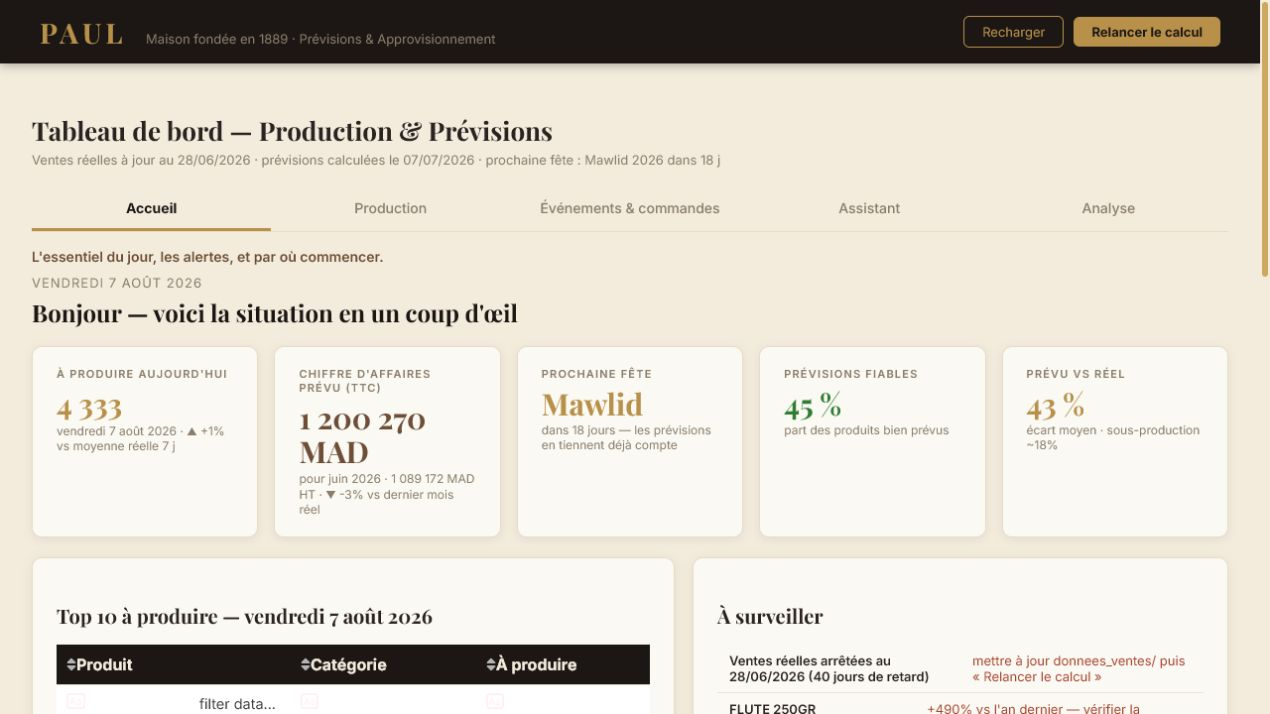
\includegraphics[width=\textwidth]{paul_accueil.png}
\caption{Page d'accueil du tableau de bord PrevisionPaul}
\label{fig:ui-accueil}
\end{figure}

\subsection{Production journalière}

La vue de production du jour affiche les quantités recommandées et permet de
choisir une date, une catégorie et un export Excel. Trois indicateurs résument le
volume du jour, le nombre de références à préparer et l'horizon disponible. La
prévision centrale et la fiabilité restent accessibles dans le tableau afin que
l'utilisateur distingue le besoin moyen de la marge de sécurité.

\begin{figure}[H]
\centering
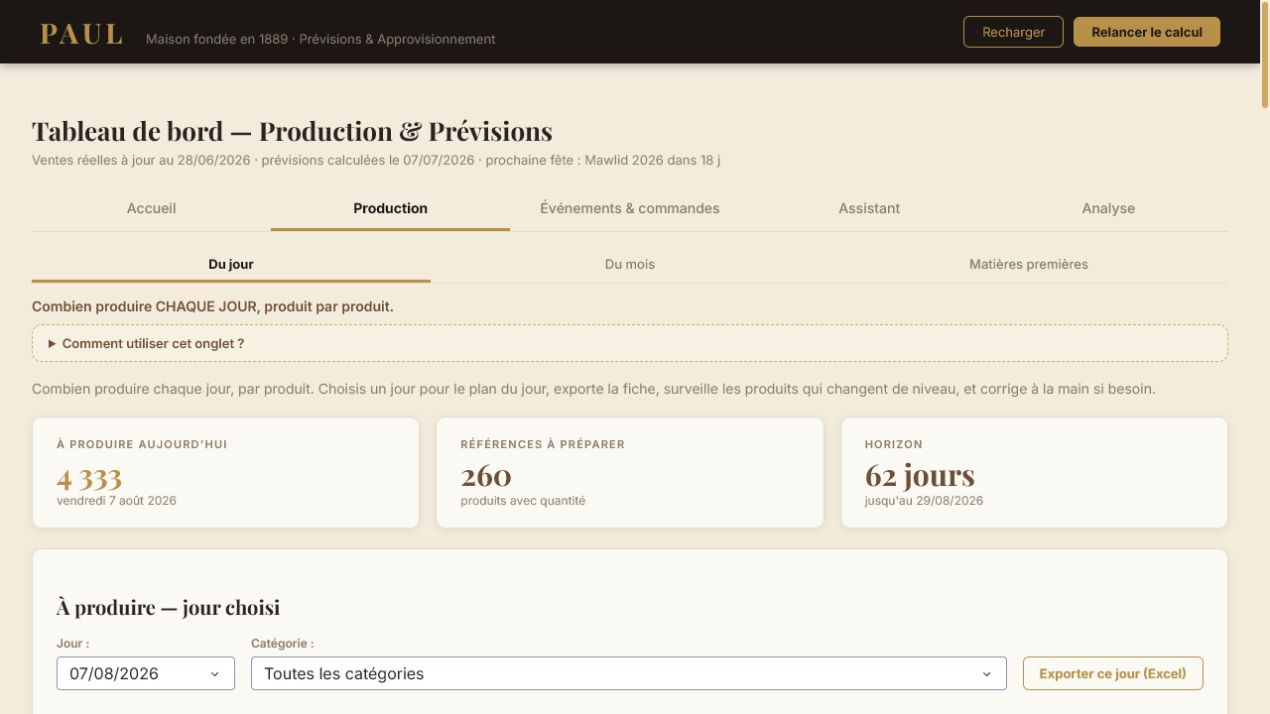
\includegraphics[width=\textwidth]{paul_production_jour.png}
\caption{Vue de production journalière}
\label{fig:ui-production}
\end{figure}

\subsection{Matières premières}

La vue MRP présente 236 ingrédients distincts pour le mois calculé. Elle regroupe
les solides, les liquides, le budget d'achat estimé, le food-cost plancher et la
couverture des prix. Le tableau détaillé permet de contrôler les matières les plus
importantes. Une seconde section classe les recettes à saisir en priorité selon le
poids matière qu'elles représentent.

\begin{figure}[H]
\centering
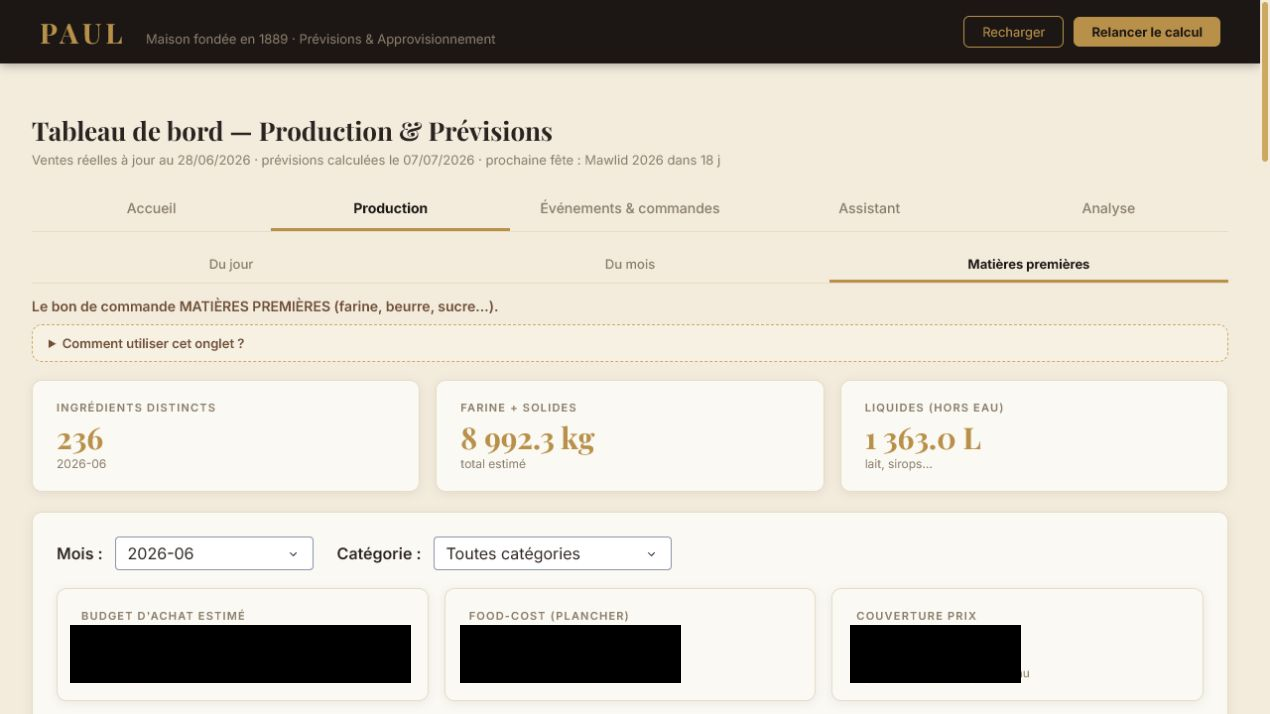
\includegraphics[width=\textwidth]{paul_matieres_premieres.png}
\caption{Vue des besoins en matières premières}
\label{fig:ui-mrp}
\end{figure}

\subsection{Événements et commandes}

L'utilisateur peut déclarer un match, un jour férié, un concert ou un autre
événement. Pour un match, l'impact est appris à partir des occurrences passées et
pondéré par l'importance de la rencontre ; pour les autres types, un impact manuel
peut être saisi. L'onglet voisin enregistre les commandes clients datées.

\begin{figure}[H]
\centering
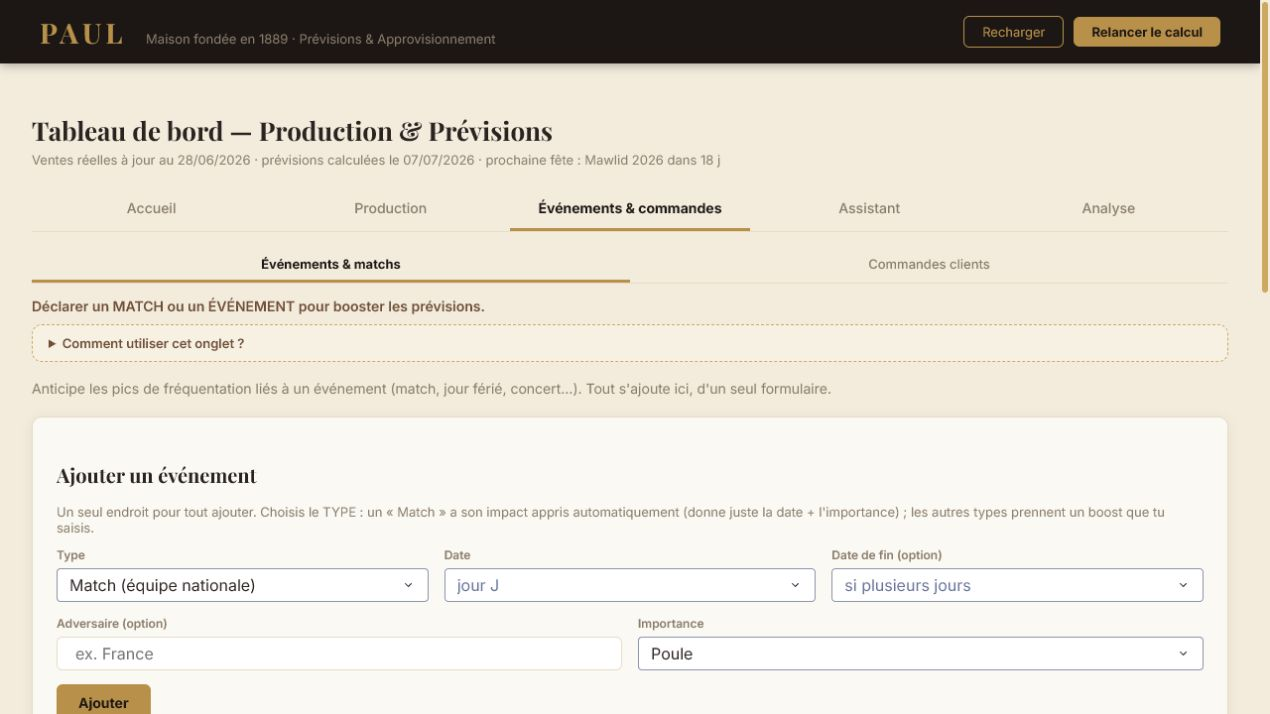
\includegraphics[width=\textwidth]{paul_evenements.png}
\caption{Gestion des événements et des matchs}
\label{fig:ui-evenements}
\end{figure}

\subsection{Assistant déterministe local}

La figure~\ref{fig:ui-assistant} montre l'assistant guidé. L'utilisateur choisit
un type de question et renseigne uniquement les champs nécessaires. La fonction
correspondante lit les fichiers réels et renvoie un texte et, si besoin, un
tableau. Ce choix privilégie la confidentialité et l'absence d'hallucination par
rapport à une conversation libre avec un service externe.

\begin{figure}[H]
\centering
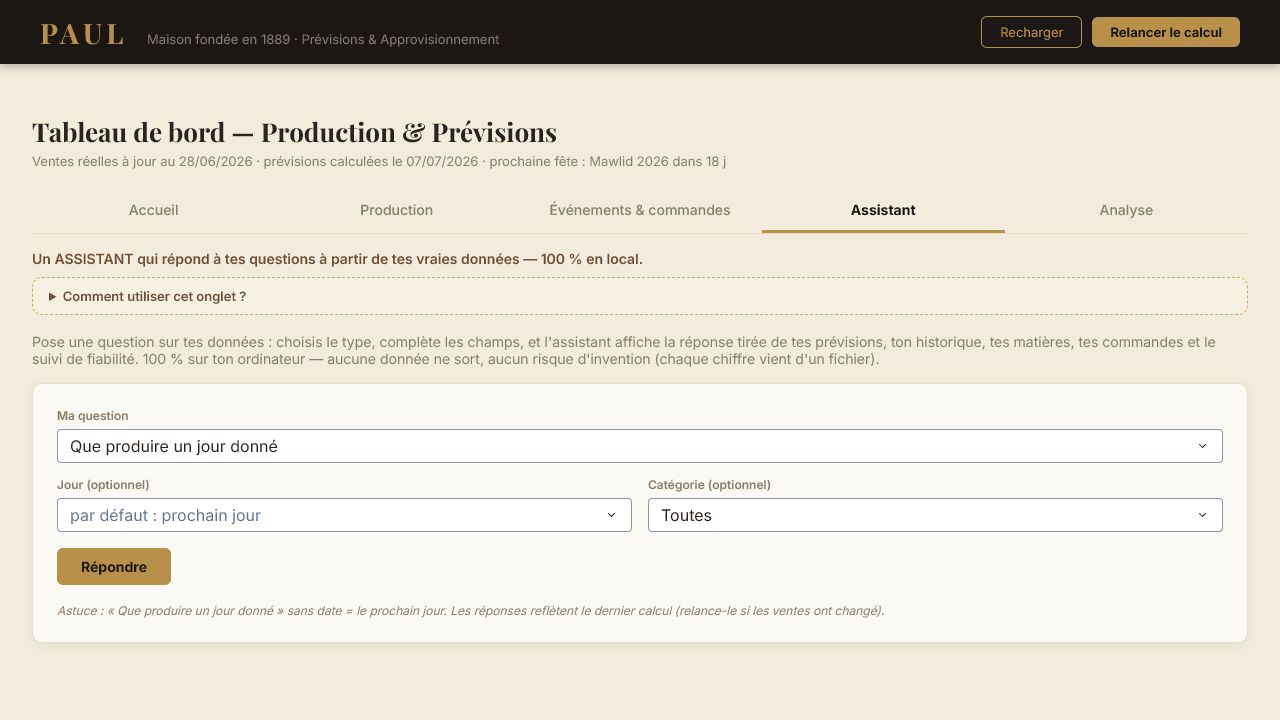
\includegraphics[width=\textwidth]{paul_assistant_local.png}
\caption{Assistant local fondé sur les données calculées}
\label{fig:ui-assistant}
\end{figure}

\subsection{Analyse du chiffre d'affaires et des marges}

L'espace Analyse rassemble l'historique, les prévisions de chiffre d'affaires et
les marges matière par produit. Les cartes indiquent notamment un chiffre
d'affaires historique HT de 51,53 millions MAD sur les données consolidées par le
dashboard, un mois moyen de 873\,399 MAD et les prévisions 2026. Les marges restent
qualifiées d'indicatives tant que toutes les recettes et tous les prix ne sont pas
validés.

\begin{figure}[H]
\centering
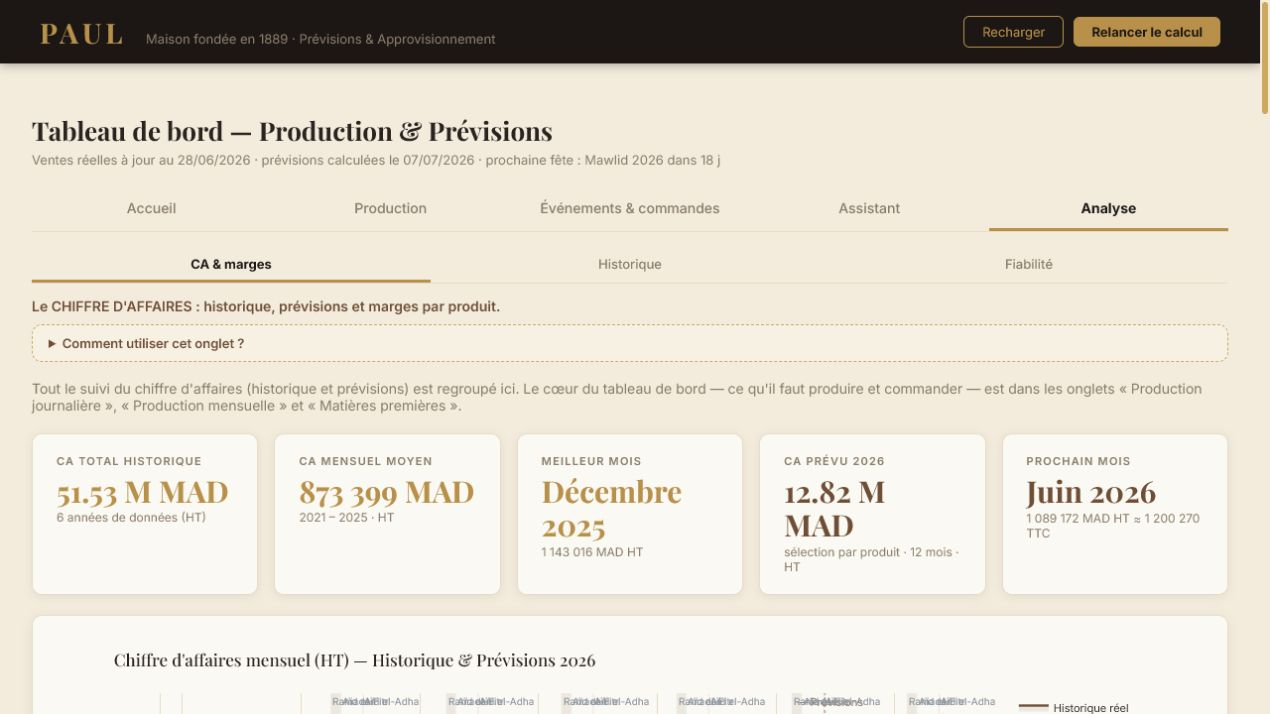
\includegraphics[width=\textwidth]{paul_analyse_marges.png}
\caption{Analyse du chiffre d'affaires et des marges matière}
\label{fig:ui-analyse}
\end{figure}

\section{Automatisation et déploiement}

Le dépôt fournit un lanceur double-clic pour l'utilisateur final et un script
d'installation de raccourci avec l'icône PAUL. En production, le code est prévu
dans \texttt{C:\textbackslash PrevisionPaul}, hors des dossiers personnels. Une
tâche Windows nommée « PrevisionPaul - MAJ quotidienne » exécute le script
\texttt{mise\_a\_jour\_quotidienne.py} à 05 h 30. Les étapes et erreurs sont
écrites dans un fichier \texttt{logs/auto\_AAAAMMJJ.log}.

Le code est synchronisé par Git, tandis que les ventes, recettes et prix sensibles
restent exclus du dépôt public. Cette séparation simplifie les mises à jour : un
\texttt{git pull} actualise l'application sans déplacer les données locales.

\section{Tests et validation}

\subsection{Stratégie de test}

La suite Pytest couvre les règles les plus sensibles : préparation des données,
prévisions, fêtes, commandes, incertitude, nomenclatures, coûts, couverture,
assistant et exports. Un test spécifique vérifie que l'assistant ne dépend
d'aucun service réseau. D'autres tests contrôlent l'ajout exact d'une commande,
la neutralisation des pics, les unités de matière et l'absence de régression dans
les tables générées.

La commande \texttt{python -m pytest tests -q} a été exécutée après la
synchronisation GitHub. Les 86 tests ont réussi en 7,85 secondes sur la machine de
validation.

\begin{resultatbox}[title=Résultat de la recette technique,fonttitle=\bfseries]
\centering
\Large\textbf{86 tests réussis sur 86}\par
\normalsize Aucun échec détecté sur le commit \texttt{be291f7}.
\end{resultatbox}

\subsection{Validation mensuelle}

La validation walk-forward disponible rejoue douze mois, de juin 2025 à mai 2026.
Elle confirme que Holt--Winters est le meilleur modèle agrégé parmi les cinq
séries de référence du fichier de validation : WAPE de 8,25\,\% sur les quantités
et 8,28\,\% sur le chiffre d'affaires. Cette mesure ne remplace pas la sélection
par produit ; elle contrôle la cohérence du niveau global.

\begin{table}[H]
\centering
\caption{Résultats de la validation mensuelle agrégée}
\label{tab:validation-mensuelle}
\begin{tabularx}{\textwidth}{Y C{3cm} C{3cm}}
\toprule
\textbf{Modèle} & \textbf{WAPE quantité} & \textbf{WAPE CA} \\
\midrule
Moyenne mobile & 9,36\,\% & 11,09\,\% \\
Tendance & 15,18\,\% & 19,03\,\% \\
Naïf saisonnier & 19,31\,\% & 22,92\,\% \\
Décomposition saisonnière & 16,22\,\% & 20,49\,\% \\
\textbf{Holt--Winters} & \textbf{8,25\,\%} & \textbf{8,28\,\%} \\
\bottomrule
\end{tabularx}
\end{table}

\begin{figure}[H]
\centering
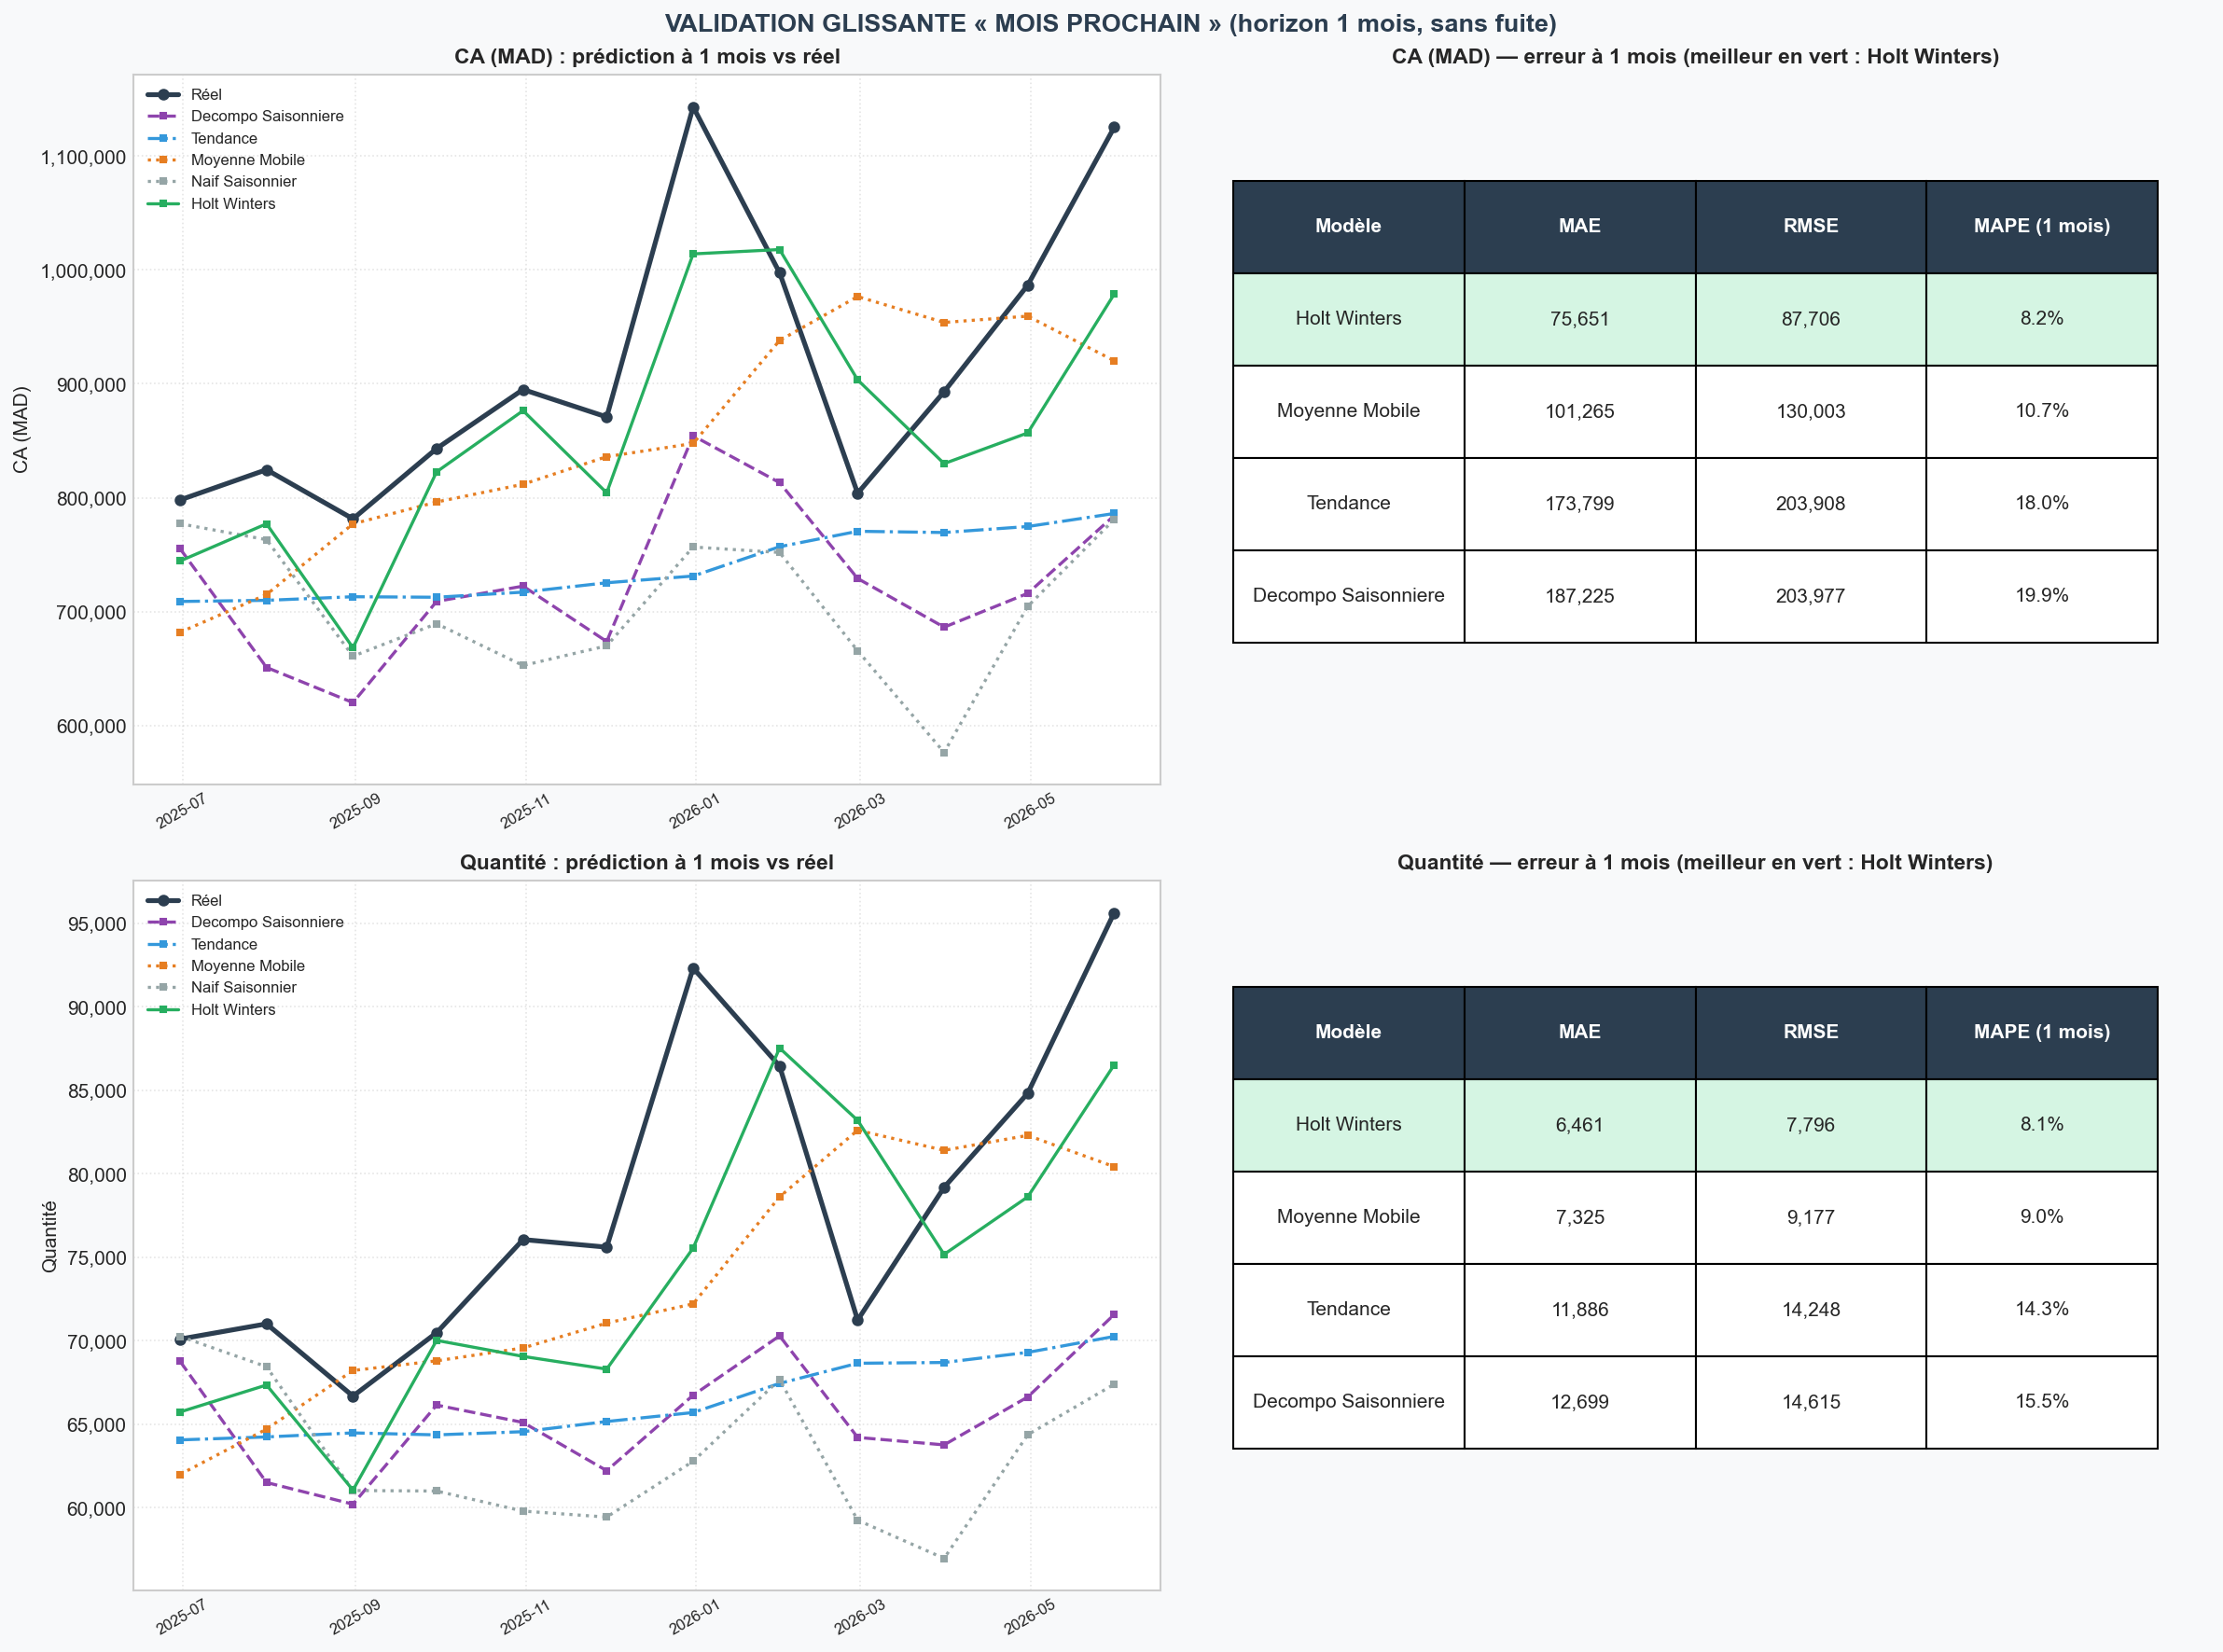
\includegraphics[width=0.92\textwidth]{dashboard_validation_mensuelle.png}
\caption{Graphique de validation mensuelle généré par le pipeline}
\label{fig:validation-mensuelle}
\end{figure}

\subsection{Suivi journalier}

Le suivi du 1\textsuperscript{er} au 28 juin 2026 contient 30\,905 comparaisons
produit-date. À l'échelle de toutes les lignes, le WAPE atteint 43,47\,\%, ce qui
reflète la difficulté de la longue traîne et des petits volumes. Après agrégation
par jour, le WAPE est de 18,62\,\% et le biais de $-18,12\,\%$, indiquant une
sous-prévision globale sur cette fenêtre. Ce diagnostic est affiché plutôt que
masqué : il justifie la marge de sécurité et la nécessité de mettre à jour les
ventes, arrêtées au 28 juin dans la capture du 7 août.

\begin{table}[H]
\centering
\caption{Indicateurs observés dans les exports du 7 juillet 2026}
\label{tab:resultats-observes}
\begin{tabularx}{\textwidth}{p{5.4cm}Y}
\toprule
\textbf{Indicateur} & \textbf{Valeur} \\
\midrule
Produits dans le plan mensuel & 1\,164 \\
Prévision mensuelle centrale totale & 95\,898 unités \\
Quantité mensuelle recommandée totale & 128\,239 unités \\
Part des lignes mensuelles classées fiables & 44,8\,\% \\
Horizon de prévision journalière & 62 jours \\
Produits dans l'export journalier & 1\,109 \\
Ingrédients distincts calculés & 236 \\
Budget matière estimé affiché & 200\,430 MAD \\
Couverture des prix affichée & 94\,\% \\
Tests automatisés & 86 / 86 réussis \\
\bottomrule
\end{tabularx}
\end{table}

\begin{attentionbox}
Les résultats chiffrés correspondent aux fichiers disponibles au 7 juillet 2026.
Ils ne constituent pas une prévision actualisée au 7 août 2026, car les ventes
réelles s'arrêtent au 28 juin. Le dashboard détecte et affiche ce retard. Une
mise à jour SQL ou fichier, suivie d'un recalcul, est nécessaire avant toute
décision opérationnelle réelle.
\end{attentionbox}

\section{Difficultés rencontrées et solutions}

\subsection{Hétérogénéité et qualité des données}

Les exports historiques combinent plusieurs années, sites, encodages et formats.
Les sous-totaux pouvaient doubler les volumes. Nous avons stabilisé un schéma CSV,
introduit des contrôles de seuil, consolidé les mois récents et conservé un
référentiel de nettoyage. Le système refuse désormais de remplacer un historique
valide par une extraction vide.

\subsection{Longue traîne et changements de régime}

Plusieurs centaines de produits ont un historique court ou intermittent. Les
modèles classiques deviennent instables et une erreur relative sur un volume
presque nul perd son sens. Nous avons combiné Croston, des replis simples, un GBM
global et des étiquettes spécifiques. Pour les références qui changent rapidement
de niveau, le modèle journalier augmente le poids de la fenêtre récente tout en
bornant la réaction à un pic isolé.

\subsection{Recettes incomplètes et unités}

La qualité du MRP dépend directement des nomenclatures. Des variations de casse,
des codes internes et des unités incohérentes empêchaient certains rapprochements.
Nous avons ajouté des alias, une normalisation des unités, une gestion récursive
des PSF et un workflow de validation par le chef. Les derniers correctifs du dépôt
traitent notamment une erreur d'échelle kilogramme/gramme et plusieurs familles de
préparations cuisine.

\subsection{Lisibilité de l'interface}

Le dashboard regroupe de nombreux usages dans un seul fichier d'application. Une
navigation plate aurait créé trop d'onglets. Nous avons donc organisé les vues en
cinq groupes, ajouté des sous-onglets thématiques, des aides contextuelles et des
cartes de navigation. Les lectures coûteuses sont mises en cache puis invalidées
après un recalcul.

\section{Conclusion}

La réalisation concrétise l'architecture décrite au chapitre précédent : sources
contrôlées, moteurs séparés, règles métier explicites, exports traçables et
interface orientée décision. Les résultats mensuels sont satisfaisants au niveau
agrégé et la suite automatisée valide les comportements critiques. Le suivi
journalier met toutefois en évidence un biais récent et rappelle qu'un outil de
prévision doit être surveillé et recalibré en continu.

\clearpage
\chapter*{Conclusion générale}
\phantomsection
\addcontentsline{toc}{chapter}{Conclusion générale}
\markboth{Conclusion générale}{Conclusion générale}
\vspace{-1\baselineskip}
{\setstretch{1.40}

L'objectif de ce projet était de transformer un historique de ventes hétérogène en
un outil local capable d'aider concrètement les équipes de PAUL Maroc à décider
quoi produire et quoi commander. Pour atteindre cet objectif, nous avons construit
une chaîne complète qui consolide les ventes journalières et mensuelles, compare
dix candidats de prévision selon le produit, réconcilie les résultats avec un
niveau global, intègre les fêtes marocaines, les matchs, les événements et les
commandes clients, puis convertit les quantités recommandées en besoins de matières
premières grâce aux recettes et aux produits semi-finis. Le résultat prend la
forme de plans quotidien et mensuel sécurisés, d'un bon de commande,
d'indicateurs de coût et d'une interface accessible. La version étudiée
traite 373\,875 lignes de ventes, couvre plus de mille produits, sélectionne un
modèle pour 848 références et calcule 236 ingrédients distincts. La validation
mensuelle glissante obtient un WAPE de 8,25\,\% sur les quantités agrégées avec
Holt--Winters, tandis que les 86 tests automatisés réussissent sur le dernier
commit synchronisé. Ces résultats montrent que l'architecture répond aux besoins
fondamentaux de reproductibilité, de traçabilité et de confidentialité. Ils doivent
cependant être interprétés avec esprit critique. La précision journalière se
dégrade sur la longue traîne et la fenêtre récente révèle une sous-prévision
globale ; les ventes disponibles lors de l'audit s'arrêtent au 28 juin 2026 ; une
partie des recettes et des prix reste estimée ; enfin, le food-cost calculé ne
comprend pas encore toutes les charges. Le dashboard rend ces limites visibles
afin que l'utilisateur ne confonde pas une recommandation avec une certitude. Les
prochaines améliorations devraient donc porter en priorité sur l'alimentation SQL
continue, la validation systématique des recettes par le chef, l'intégration des
stocks réels et des délais fournisseurs, le suivi de la casse et des invendus, et
la mise en place d'alertes lorsque le biais dépasse un seuil. Une évolution vers
un stockage relationnel des configurations et des historiques d'exécution
faciliterait également le multi-site et la gestion des droits. Enfin, un modèle
local de langage pourrait enrichir l'assistant en langage naturel, à condition de
conserver les outils déterministes comme seule source de chiffres et de ne jamais
faire sortir les données de l'entreprise. Ce projet nous a permis d'articuler
ingénierie logicielle, données, séries temporelles et contraintes opérationnelles.
\par}

\clearpage
\renewcommand{\bibname}{Bibliographie et nétographie}
\phantomsection
\addcontentsline{toc}{chapter}{Bibliographie et nétographie}
\markboth{Bibliographie et nétographie}{Bibliographie et nétographie}
\begin{thebibliography}{99}

\addcontentsline{toc}{section}{Bibliographie}

\bibitem{hyndman2021}
HYNDMAN, Rob J. et ATHANASOPOULOS, George.
\textit{Forecasting: Principles and Practice}, 3\textsuperscript{e} édition,
Melbourne, OTexts, 2021. Version en ligne consultée le 7 août 2026 :
\url{https://otexts.com/fpp3/}.

\bibitem{omgUML}
OBJECT MANAGEMENT GROUP.
\textit{OMG Unified Modeling Language, Version 2.5.1}, décembre 2017.
Spécification consultée le 7 août 2026 :
\url{https://www.omg.org/spec/UML/2.5.1}.

\bibitem{rapportInterne}
ÉCOLE MAROCAINE DES SCIENCES DE L'INGÉNIEUR.
\textit{Template du rapport de projet de fin d'année — 4e année IIR},
document pédagogique interne, année universitaire 2025--2026.

\section*{Nétographie et documentation technique}

\bibitem{pandasDocs}
PANDAS DEVELOPMENT TEAM.
\textit{pandas User Guide}. Documentation officielle consultée le 7 août 2026 :
\url{https://pandas.pydata.org/docs/user_guide/}.

\bibitem{statsmodelsHW}
STATSMODELS DEVELOPERS.
\textit{statsmodels.tsa.holtwinters.ExponentialSmoothing}.
Documentation officielle consultée le 7 août 2026 :
\url{https://www.statsmodels.org/dev/generated/statsmodels.tsa.holtwinters.ExponentialSmoothing}.

\bibitem{sklearnGBM}
SCIKIT-LEARN DEVELOPERS.
\textit{GradientBoostingRegressor}. Documentation officielle consultée le
7 août 2026 :
\url{https://scikit-learn.org/stable/modules/generated/sklearn.ensemble.GradientBoostingRegressor.html}.

\bibitem{dashDocs}
PLOTLY.
\textit{Dash for Python Documentation — Layout}.
Documentation officielle consultée le 7 août 2026 :
\url{https://dash.plotly.com/layout}.

\bibitem{repo}
MOUSSAWI, Othmane.
\textit{PrevisionPaul — dépôt du projet}.
Version \texttt{be291f7}, consultée le 7 août 2026 :
\url{https://github.com/OthmaneW37/PrevisionPaul}.

\end{thebibliography}

\clearpage
\appendix

\newcommand{\annexepage}[1]{%
  \clearpage
  \refstepcounter{chapter}
  \phantomsection
  \addcontentsline{toc}{chapter}{Annexe \thechapter{} : #1}
  \markboth{Annexe \thechapter{} — #1}{Annexe \thechapter{} — #1}
  \thispagestyle{empty}
  \vspace*{3.2cm}
  \begin{center}
    {\LARGE\bfseries Annexe \thechapter\par}
    \vspace{1cm}
    {\color{paulGold}\rule{\textwidth}{1pt}}\\[1.2cm]
    {\Huge\bfseries #1\par}
    \vspace{1.2cm}
    {\color{paulGold}\rule{\textwidth}{1pt}}
  \end{center}
  \vfill
  \begin{center}\color{gray}\NomProjet\end{center}
  \clearpage}

\annexepage{Guide d'installation et d'exploitation}

\section{Installation locale}

Le code et les données doivent être séparés. Le code peut être cloné depuis le
dépôt, tandis que les dossiers sensibles sont transférés directement sur la
machine de l'entreprise.

\begin{lstlisting}[style=paulpython,language=bash,caption={Commandes d'installation}]
git clone https://github.com/OthmaneW37/PrevisionPaul.git
cd PrevisionPaul
python -m pip install -r requirements.txt
python -m pytest tests -q
\end{lstlisting}

Les dossiers \texttt{data/} et \texttt{donnees\_ventes/} doivent ensuite être
placés dans la racine du projet. Ils ne sont pas publiés avec le code lorsqu'ils
contiennent des informations métier.

\section{Commandes d'exploitation}

\small
\begin{longtable}{p{6.8cm}p{7.4cm}}
\caption{Principales commandes d'exploitation}\label{tab:commandes-exploitation}\\
\toprule
\textbf{Commande} & \textbf{Effet} \\
\midrule
\endfirsthead
\toprule
\textbf{Commande} & \textbf{Effet} \\
\midrule
\endhead
\path{python dashboard.py} & Lance le tableau de bord sur \url{http://127.0.0.1:8050}. \\
\path{python main.py} & Recalcule les prévisions mensuelles, le plan sécurisé et le MRP. \\
\path{python -m paul_forecast.forecast_journalier} & Régénère l'horizon journalier de 62 jours. \\
\path{python outils/exporter_ventes_sql.py} & Lit les jours clôturés depuis SQL Server et fusionne le CSV. \\
\path{python outils/mise_a_jour_quotidienne.py} & Exécute export SQL, journalier puis mensuel avec journalisation. \\
\path{python outils/generer_tableau_recettes.py} & Crée le classeur à compléter par le chef. \\
\path{python outils/importer_recettes_chefs.py} & Importe les recettes explicitement validées. \\
\path{python -m pytest tests -q} & Lance l'ensemble des tests automatisés. \\
\bottomrule
\end{longtable}
\normalsize

\section{Procédure de mise à jour quotidienne}

\begin{enumerate}
  \item vérifier que la base Elyx est accessible ou déposer le nouvel export dans
  \path{donnees_ventes/} ;
  \item lancer la chaîne quotidienne ou attendre la tâche de 05 h 30 ;
  \item consulter le journal du jour dans \texttt{logs/} ;
  \item ouvrir le dashboard et contrôler la date « ventes réelles à jour au » ;
  \item examiner les alertes de niveau et la fiabilité avant d'exporter le plan ;
  \item vérifier le bon de commande avec le chef lorsque des recettes sont encore
  estimées.
\end{enumerate}

\annexepage{Structure du projet et fichiers produits}

\section{Arborescence fonctionnelle}

\begin{lstlisting}[basicstyle=\ttfamily\small,frame=single,backgroundcolor=\color{softGray}]
PrevisionPaul/
|-- dashboard.py              # interface Dash
|-- main.py                   # point d'entree mensuel
|-- watcher.py                # surveillance des fichiers
|-- paul_forecast/            # moteurs et regles metier
|-- data/                     # configuration JSON locale
|-- donnees_ventes/           # historique des ventes
|-- exports/                  # sorties journalieres et datees
|-- outils/                   # imports, benchmarks, recettes
|-- tests/                    # suite Pytest
|-- docs/                     # documents pour les equipes
`-- Rapport/                  # sources LaTeX du present rapport
\end{lstlisting}

\section{Exports principaux}

\small
\begin{longtable}{p{7.0cm}p{7.2cm}}
\caption{Fichiers produits par le système}\label{tab:exports}\\
\toprule
\textbf{Fichier} & \textbf{Contenu} \\
\midrule
\endfirsthead
\toprule
\textbf{Fichier} & \textbf{Contenu} \\
\midrule
\endhead
\path{exports/previsions_journalieres.csv} & Date, produit, famille, prévision, recommandation, fiabilité et commande. \\
\path{exports/suivi_prevu_reel.csv} & Comparaison hors échantillon sur les jours récents. \\
\path{plan_production_securise.csv} & Plan mensuel par produit, modèle, erreur et intervalle. \\
\path{besoins_ingredients_planifies.csv} & Quantité requise par ingrédient et par mois. \\
\path{previsions_detaillees_par_produit.csv} & Historique et scénarios de prévision détaillés. \\
\path{previsions_par_famille.csv} & Synthèse mensuelle par famille. \\
\path{validation_mensuelle_quantite.csv} & Réel et prévisions walk-forward en quantité. \\
\path{validation_mensuelle_ca.csv} & Réel et prévisions walk-forward en chiffre d'affaires. \\
\path{previsions_PAUL_2026.xlsx} & Classeur multi-feuilles à destination du responsable. \\
\path{bon_de_commande_gerant.txt} & Synthèse textuelle des matières à commander. \\
\bottomrule
\end{longtable}
\normalsize

\annexepage{Compléments de validation}

\section{Répartition des modèles sélectionnés}

Le benchmark disponible contient 848 produits. La répartition du meilleur modèle
montre l'intérêt d'une sélection hétérogène : Theta est retenu pour 293 produits,
le GBM pour 227, le naïf saisonnier pour 102, ETS pour 77, la moyenne mobile pour
44, l'ensemble médian pour 35, la moyenne pour 23, ARIMA pour 20, Croston pour 14
et l'ensemble moyen pour 13.

\begin{table}[H]
\centering
\caption{Répartition des modèles retenus dans le benchmark}
\label{tab:repartition-modeles}
\begin{tabular}{lrr@{\hspace{1.2cm}}lrr}
\toprule
\textbf{Modèle} & \textbf{Produits} & \textbf{Part} & \textbf{Modèle} & \textbf{Produits} & \textbf{Part} \\
\midrule
Theta & 293 & 34,6\,\% & Moyenne mobile & 44 & 5,2\,\% \\
GBM & 227 & 26,8\,\% & Ensemble médian & 35 & 4,1\,\% \\
Naïf saisonnier & 102 & 12,0\,\% & Moyenne & 23 & 2,7\,\% \\
ETS & 77 & 9,1\,\% & ARIMA & 20 & 2,4\,\% \\
Croston & 14 & 1,7\,\% & Ensemble moyen & 13 & 1,5\,\% \\
\bottomrule
\end{tabular}
\end{table}

\section{Graphiques statiques générés}

\begin{figure}[H]
\centering
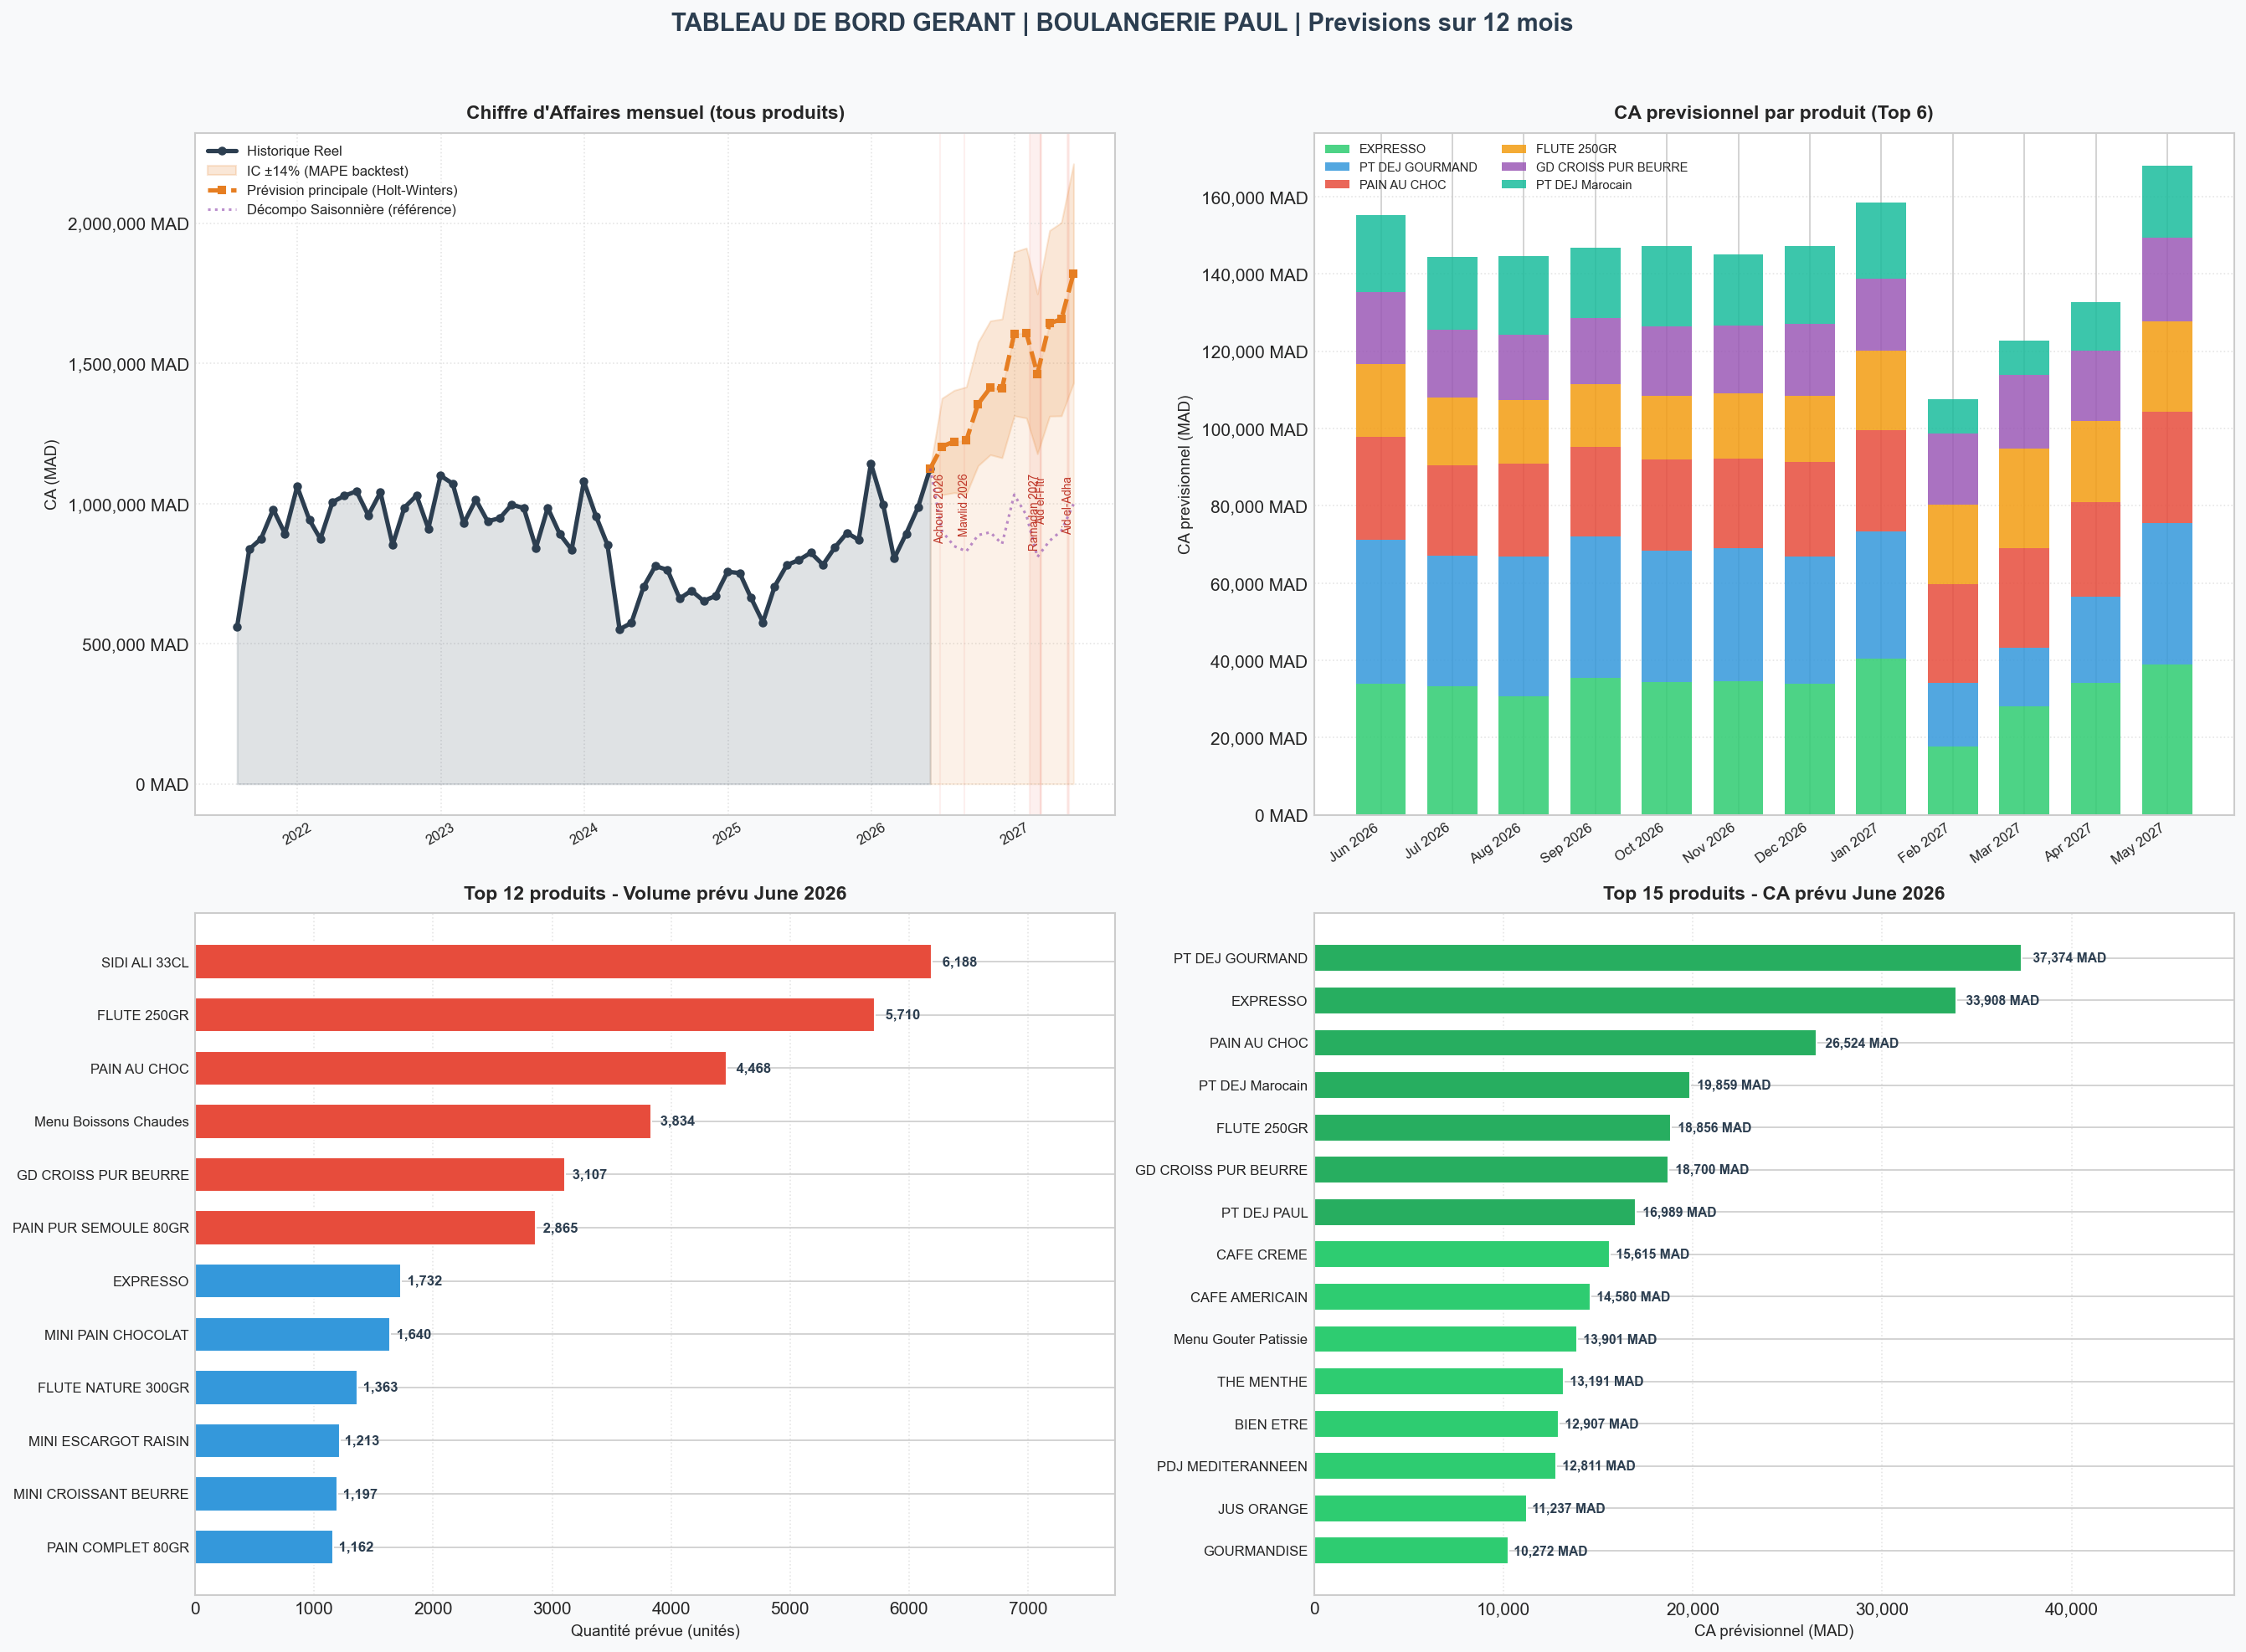
\includegraphics[width=0.92\textwidth]{dashboard_gerant.png}
\caption{Dashboard statique destiné au responsable}
\label{fig:annexe-dashboard-gerant}
\end{figure}

\begin{figure}[H]
\centering
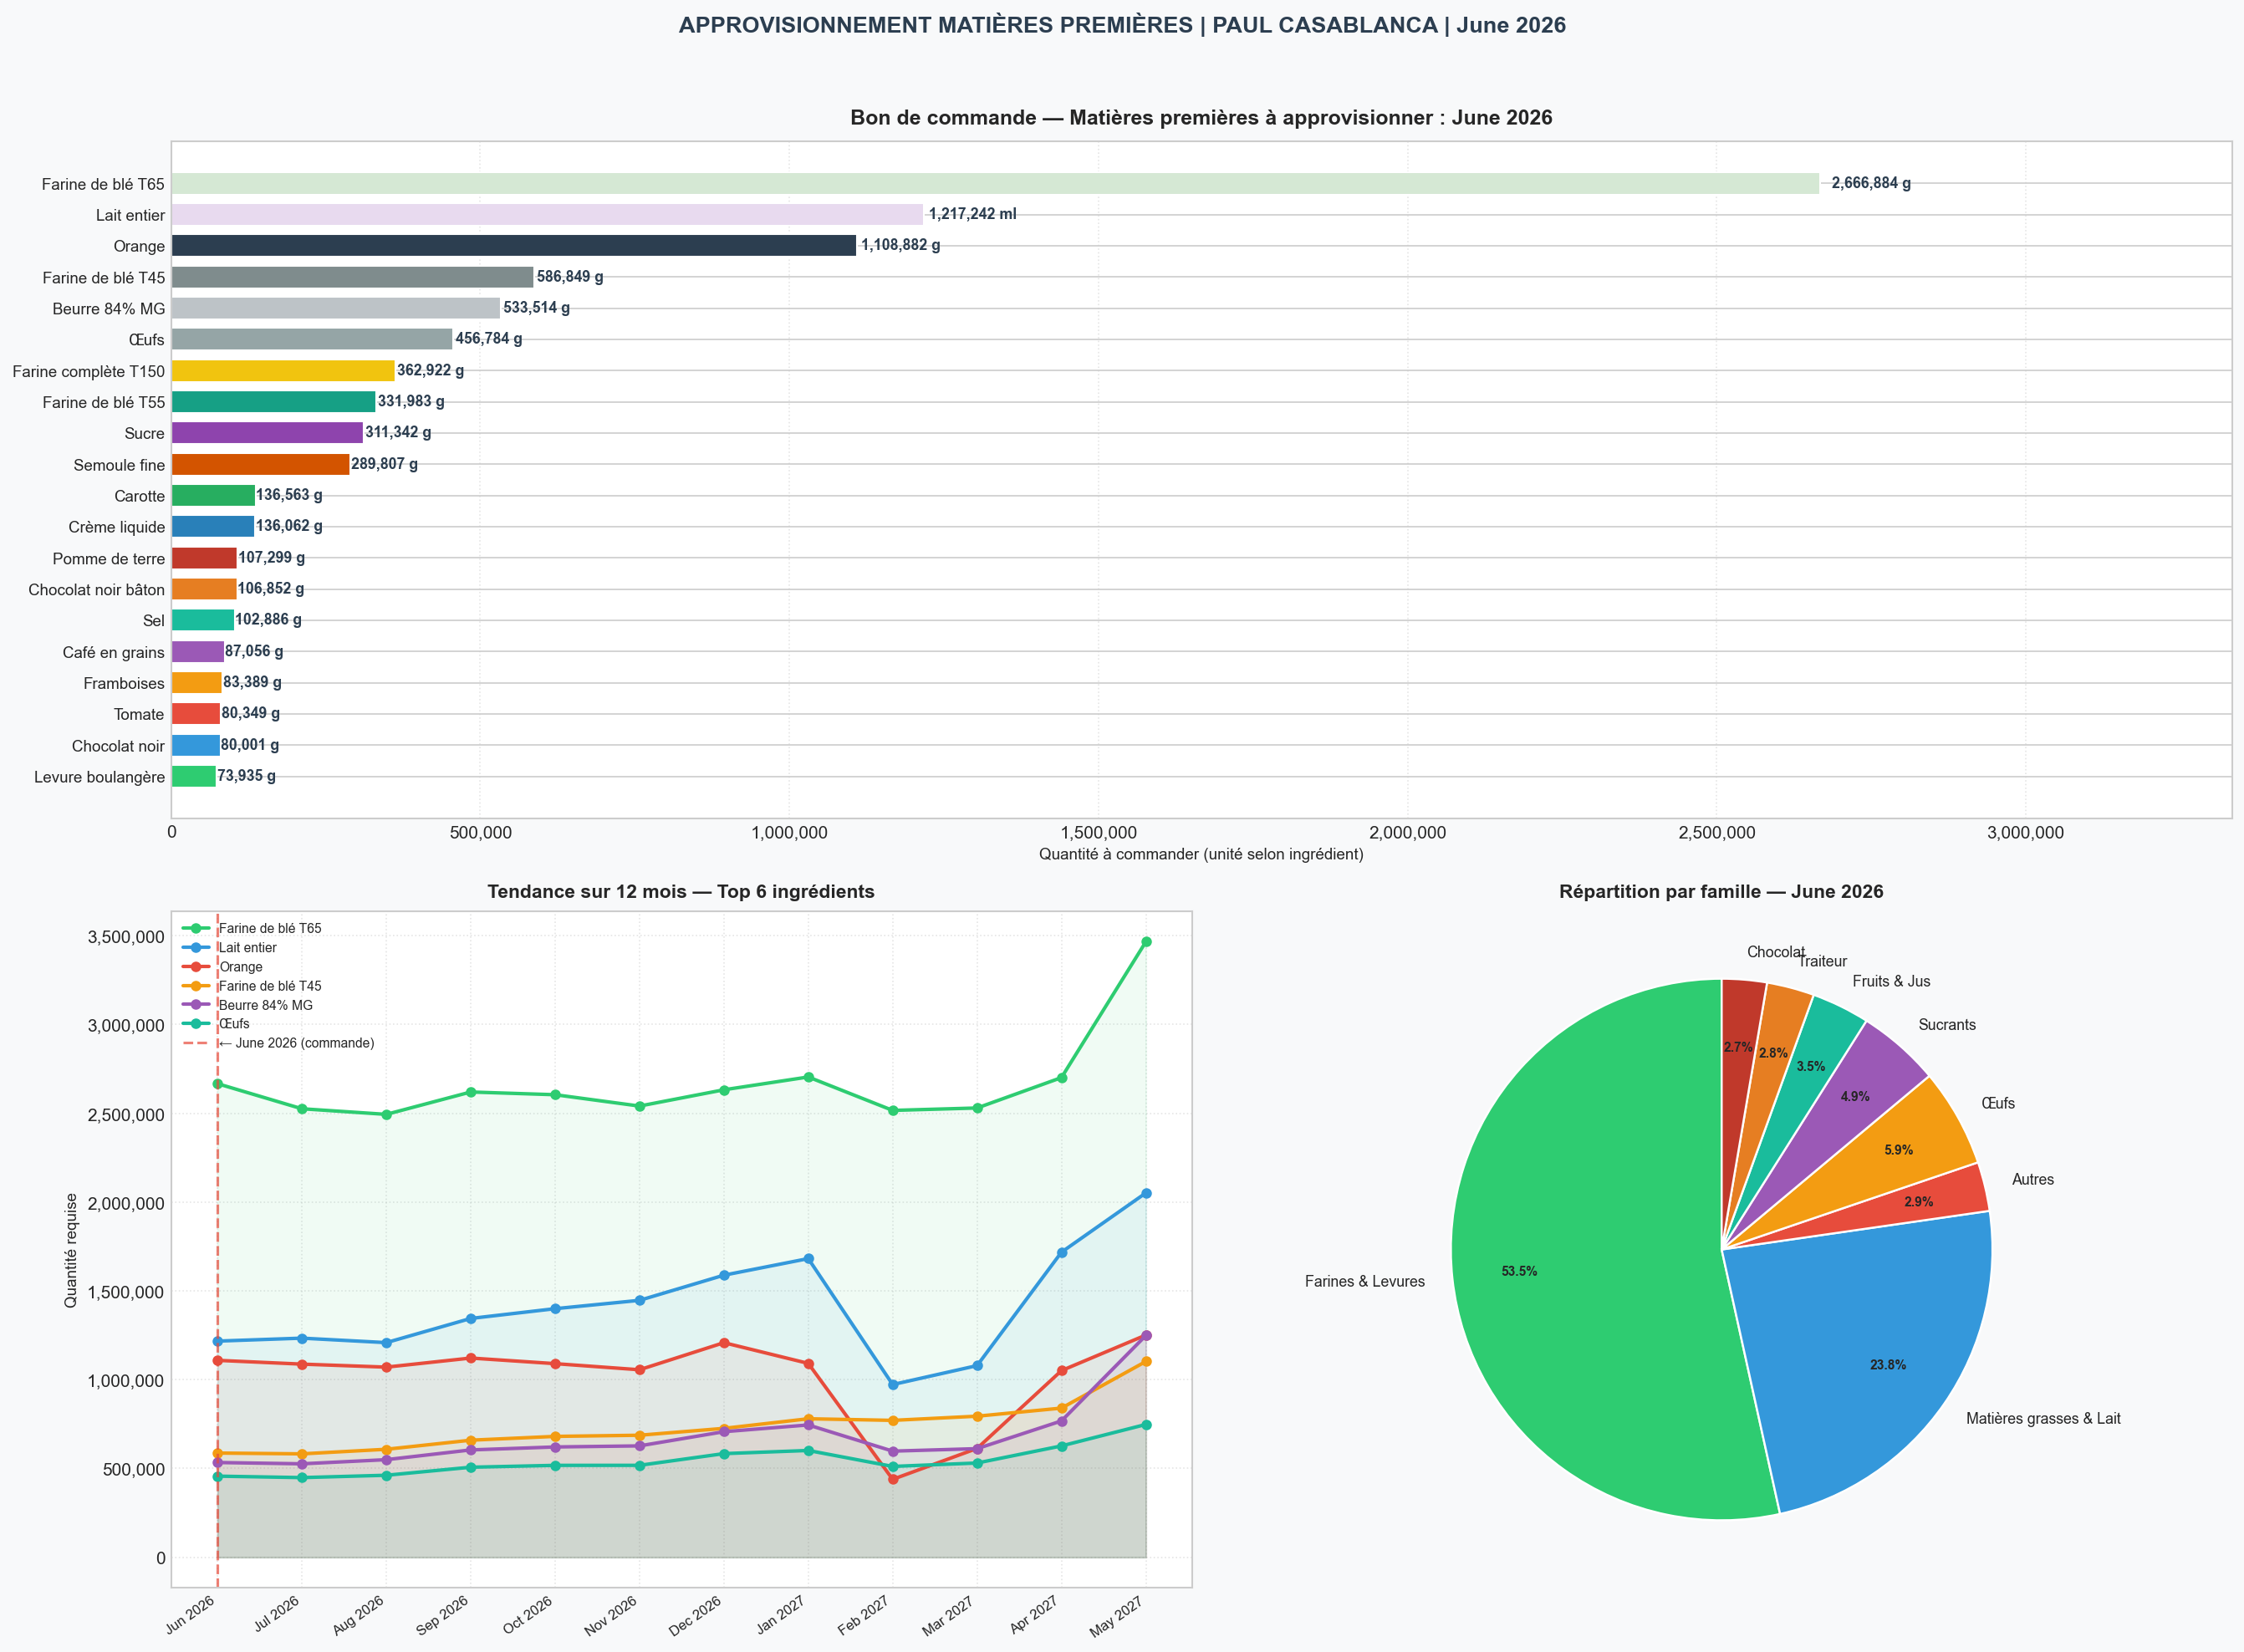
\includegraphics[width=0.92\textwidth]{dashboard_matieres_premieres.png}
\caption{Dashboard statique des matières premières}
\label{fig:annexe-dashboard-matieres}
\end{figure}

\section{Limites à contrôler avant usage opérationnel}

\begin{itemize}
  \item actualiser les ventes et vérifier la date de fraîcheur ;
  \item confirmer les recettes à plus fort poids matière ;
  \item remplacer les prix estimés par les factures fournisseurs ;
  \item retirer le calibrage provisoire des farines après validation complète ;
  \item analyser le biais journalier et recalibrer les seuils si nécessaire ;
  \item ne pas interpréter les marges matière comme une marge nette ;
  \item contrôler les événements et commandes futurs avant chaque recalcul.
\end{itemize}


\end{document}
